% Options for packages loaded elsewhere
\PassOptionsToPackage{unicode}{hyperref}
\PassOptionsToPackage{hyphens}{url}
\PassOptionsToPackage{dvipsnames,svgnames,x11names}{xcolor}
%
\documentclass[
  letterpaper,
  DIV=11,
  numbers=noendperiod]{scrreprt}

\usepackage{amsmath,amssymb}
\usepackage{iftex}
\ifPDFTeX
  \usepackage[T1]{fontenc}
  \usepackage[utf8]{inputenc}
  \usepackage{textcomp} % provide euro and other symbols
\else % if luatex or xetex
  \usepackage{unicode-math}
  \defaultfontfeatures{Scale=MatchLowercase}
  \defaultfontfeatures[\rmfamily]{Ligatures=TeX,Scale=1}
\fi
\usepackage{lmodern}
\ifPDFTeX\else  
    % xetex/luatex font selection
\fi
% Use upquote if available, for straight quotes in verbatim environments
\IfFileExists{upquote.sty}{\usepackage{upquote}}{}
\IfFileExists{microtype.sty}{% use microtype if available
  \usepackage[]{microtype}
  \UseMicrotypeSet[protrusion]{basicmath} % disable protrusion for tt fonts
}{}
\makeatletter
\@ifundefined{KOMAClassName}{% if non-KOMA class
  \IfFileExists{parskip.sty}{%
    \usepackage{parskip}
  }{% else
    \setlength{\parindent}{0pt}
    \setlength{\parskip}{6pt plus 2pt minus 1pt}}
}{% if KOMA class
  \KOMAoptions{parskip=half}}
\makeatother
\usepackage{xcolor}
\setlength{\emergencystretch}{3em} % prevent overfull lines
\setcounter{secnumdepth}{2}
% Make \paragraph and \subparagraph free-standing
\makeatletter
\ifx\paragraph\undefined\else
  \let\oldparagraph\paragraph
  \renewcommand{\paragraph}{
    \@ifstar
      \xxxParagraphStar
      \xxxParagraphNoStar
  }
  \newcommand{\xxxParagraphStar}[1]{\oldparagraph*{#1}\mbox{}}
  \newcommand{\xxxParagraphNoStar}[1]{\oldparagraph{#1}\mbox{}}
\fi
\ifx\subparagraph\undefined\else
  \let\oldsubparagraph\subparagraph
  \renewcommand{\subparagraph}{
    \@ifstar
      \xxxSubParagraphStar
      \xxxSubParagraphNoStar
  }
  \newcommand{\xxxSubParagraphStar}[1]{\oldsubparagraph*{#1}\mbox{}}
  \newcommand{\xxxSubParagraphNoStar}[1]{\oldsubparagraph{#1}\mbox{}}
\fi
\makeatother

\usepackage{color}
\usepackage{fancyvrb}
\newcommand{\VerbBar}{|}
\newcommand{\VERB}{\Verb[commandchars=\\\{\}]}
\DefineVerbatimEnvironment{Highlighting}{Verbatim}{commandchars=\\\{\}}
% Add ',fontsize=\small' for more characters per line
\usepackage{framed}
\definecolor{shadecolor}{RGB}{241,243,245}
\newenvironment{Shaded}{\begin{snugshade}}{\end{snugshade}}
\newcommand{\AlertTok}[1]{\textcolor[rgb]{0.68,0.00,0.00}{#1}}
\newcommand{\AnnotationTok}[1]{\textcolor[rgb]{0.37,0.37,0.37}{#1}}
\newcommand{\AttributeTok}[1]{\textcolor[rgb]{0.40,0.45,0.13}{#1}}
\newcommand{\BaseNTok}[1]{\textcolor[rgb]{0.68,0.00,0.00}{#1}}
\newcommand{\BuiltInTok}[1]{\textcolor[rgb]{0.00,0.23,0.31}{#1}}
\newcommand{\CharTok}[1]{\textcolor[rgb]{0.13,0.47,0.30}{#1}}
\newcommand{\CommentTok}[1]{\textcolor[rgb]{0.37,0.37,0.37}{#1}}
\newcommand{\CommentVarTok}[1]{\textcolor[rgb]{0.37,0.37,0.37}{\textit{#1}}}
\newcommand{\ConstantTok}[1]{\textcolor[rgb]{0.56,0.35,0.01}{#1}}
\newcommand{\ControlFlowTok}[1]{\textcolor[rgb]{0.00,0.23,0.31}{\textbf{#1}}}
\newcommand{\DataTypeTok}[1]{\textcolor[rgb]{0.68,0.00,0.00}{#1}}
\newcommand{\DecValTok}[1]{\textcolor[rgb]{0.68,0.00,0.00}{#1}}
\newcommand{\DocumentationTok}[1]{\textcolor[rgb]{0.37,0.37,0.37}{\textit{#1}}}
\newcommand{\ErrorTok}[1]{\textcolor[rgb]{0.68,0.00,0.00}{#1}}
\newcommand{\ExtensionTok}[1]{\textcolor[rgb]{0.00,0.23,0.31}{#1}}
\newcommand{\FloatTok}[1]{\textcolor[rgb]{0.68,0.00,0.00}{#1}}
\newcommand{\FunctionTok}[1]{\textcolor[rgb]{0.28,0.35,0.67}{#1}}
\newcommand{\ImportTok}[1]{\textcolor[rgb]{0.00,0.46,0.62}{#1}}
\newcommand{\InformationTok}[1]{\textcolor[rgb]{0.37,0.37,0.37}{#1}}
\newcommand{\KeywordTok}[1]{\textcolor[rgb]{0.00,0.23,0.31}{\textbf{#1}}}
\newcommand{\NormalTok}[1]{\textcolor[rgb]{0.00,0.23,0.31}{#1}}
\newcommand{\OperatorTok}[1]{\textcolor[rgb]{0.37,0.37,0.37}{#1}}
\newcommand{\OtherTok}[1]{\textcolor[rgb]{0.00,0.23,0.31}{#1}}
\newcommand{\PreprocessorTok}[1]{\textcolor[rgb]{0.68,0.00,0.00}{#1}}
\newcommand{\RegionMarkerTok}[1]{\textcolor[rgb]{0.00,0.23,0.31}{#1}}
\newcommand{\SpecialCharTok}[1]{\textcolor[rgb]{0.37,0.37,0.37}{#1}}
\newcommand{\SpecialStringTok}[1]{\textcolor[rgb]{0.13,0.47,0.30}{#1}}
\newcommand{\StringTok}[1]{\textcolor[rgb]{0.13,0.47,0.30}{#1}}
\newcommand{\VariableTok}[1]{\textcolor[rgb]{0.07,0.07,0.07}{#1}}
\newcommand{\VerbatimStringTok}[1]{\textcolor[rgb]{0.13,0.47,0.30}{#1}}
\newcommand{\WarningTok}[1]{\textcolor[rgb]{0.37,0.37,0.37}{\textit{#1}}}

\providecommand{\tightlist}{%
  \setlength{\itemsep}{0pt}\setlength{\parskip}{0pt}}\usepackage{longtable,booktabs,array}
\usepackage{calc} % for calculating minipage widths
% Correct order of tables after \paragraph or \subparagraph
\usepackage{etoolbox}
\makeatletter
\patchcmd\longtable{\par}{\if@noskipsec\mbox{}\fi\par}{}{}
\makeatother
% Allow footnotes in longtable head/foot
\IfFileExists{footnotehyper.sty}{\usepackage{footnotehyper}}{\usepackage{footnote}}
\makesavenoteenv{longtable}
\usepackage{graphicx}
\makeatletter
\newsavebox\pandoc@box
\newcommand*\pandocbounded[1]{% scales image to fit in text height/width
  \sbox\pandoc@box{#1}%
  \Gscale@div\@tempa{\textheight}{\dimexpr\ht\pandoc@box+\dp\pandoc@box\relax}%
  \Gscale@div\@tempb{\linewidth}{\wd\pandoc@box}%
  \ifdim\@tempb\p@<\@tempa\p@\let\@tempa\@tempb\fi% select the smaller of both
  \ifdim\@tempa\p@<\p@\scalebox{\@tempa}{\usebox\pandoc@box}%
  \else\usebox{\pandoc@box}%
  \fi%
}
% Set default figure placement to htbp
\def\fps@figure{htbp}
\makeatother
% definitions for citeproc citations
\NewDocumentCommand\citeproctext{}{}
\NewDocumentCommand\citeproc{mm}{%
  \begingroup\def\citeproctext{#2}\cite{#1}\endgroup}
\makeatletter
 % allow citations to break across lines
 \let\@cite@ofmt\@firstofone
 % avoid brackets around text for \cite:
 \def\@biblabel#1{}
 \def\@cite#1#2{{#1\if@tempswa , #2\fi}}
\makeatother
\newlength{\cslhangindent}
\setlength{\cslhangindent}{1.5em}
\newlength{\csllabelwidth}
\setlength{\csllabelwidth}{3em}
\newenvironment{CSLReferences}[2] % #1 hanging-indent, #2 entry-spacing
 {\begin{list}{}{%
  \setlength{\itemindent}{0pt}
  \setlength{\leftmargin}{0pt}
  \setlength{\parsep}{0pt}
  % turn on hanging indent if param 1 is 1
  \ifodd #1
   \setlength{\leftmargin}{\cslhangindent}
   \setlength{\itemindent}{-1\cslhangindent}
  \fi
  % set entry spacing
  \setlength{\itemsep}{#2\baselineskip}}}
 {\end{list}}
\usepackage{calc}
\newcommand{\CSLBlock}[1]{\hfill\break\parbox[t]{\linewidth}{\strut\ignorespaces#1\strut}}
\newcommand{\CSLLeftMargin}[1]{\parbox[t]{\csllabelwidth}{\strut#1\strut}}
\newcommand{\CSLRightInline}[1]{\parbox[t]{\linewidth - \csllabelwidth}{\strut#1\strut}}
\newcommand{\CSLIndent}[1]{\hspace{\cslhangindent}#1}

\KOMAoption{captions}{tableheading}
\makeatletter
\@ifpackageloaded{tcolorbox}{}{\usepackage[skins,breakable]{tcolorbox}}
\@ifpackageloaded{fontawesome5}{}{\usepackage{fontawesome5}}
\definecolor{quarto-callout-color}{HTML}{909090}
\definecolor{quarto-callout-note-color}{HTML}{0758E5}
\definecolor{quarto-callout-important-color}{HTML}{CC1914}
\definecolor{quarto-callout-warning-color}{HTML}{EB9113}
\definecolor{quarto-callout-tip-color}{HTML}{00A047}
\definecolor{quarto-callout-caution-color}{HTML}{FC5300}
\definecolor{quarto-callout-color-frame}{HTML}{acacac}
\definecolor{quarto-callout-note-color-frame}{HTML}{4582ec}
\definecolor{quarto-callout-important-color-frame}{HTML}{d9534f}
\definecolor{quarto-callout-warning-color-frame}{HTML}{f0ad4e}
\definecolor{quarto-callout-tip-color-frame}{HTML}{02b875}
\definecolor{quarto-callout-caution-color-frame}{HTML}{fd7e14}
\makeatother
\makeatletter
\@ifpackageloaded{bookmark}{}{\usepackage{bookmark}}
\makeatother
\makeatletter
\@ifpackageloaded{caption}{}{\usepackage{caption}}
\AtBeginDocument{%
\ifdefined\contentsname
  \renewcommand*\contentsname{Table of contents}
\else
  \newcommand\contentsname{Table of contents}
\fi
\ifdefined\listfigurename
  \renewcommand*\listfigurename{List of Figures}
\else
  \newcommand\listfigurename{List of Figures}
\fi
\ifdefined\listtablename
  \renewcommand*\listtablename{List of Tables}
\else
  \newcommand\listtablename{List of Tables}
\fi
\ifdefined\figurename
  \renewcommand*\figurename{Figure}
\else
  \newcommand\figurename{Figure}
\fi
\ifdefined\tablename
  \renewcommand*\tablename{Table}
\else
  \newcommand\tablename{Table}
\fi
}
\@ifpackageloaded{float}{}{\usepackage{float}}
\floatstyle{ruled}
\@ifundefined{c@chapter}{\newfloat{codelisting}{h}{lop}}{\newfloat{codelisting}{h}{lop}[chapter]}
\floatname{codelisting}{Listing}
\newcommand*\listoflistings{\listof{codelisting}{List of Listings}}
\usepackage{amsthm}
\theoremstyle{remark}
\AtBeginDocument{\renewcommand*{\proofname}{Proof}}
\newtheorem*{remark}{Remark}
\newtheorem*{solution}{Solution}
\newtheorem{refremark}{Remark}[chapter]
\newtheorem{refsolution}{Solution}[chapter]
\makeatother
\makeatletter
\makeatother
\makeatletter
\@ifpackageloaded{caption}{}{\usepackage{caption}}
\@ifpackageloaded{subcaption}{}{\usepackage{subcaption}}
\makeatother

\usepackage{bookmark}

\IfFileExists{xurl.sty}{\usepackage{xurl}}{} % add URL line breaks if available
\urlstyle{same} % disable monospaced font for URLs
\hypersetup{
  pdftitle={DATA 545 Tutorial},
  pdfauthor={Stacy DeRuiter},
  colorlinks=true,
  linkcolor={blue},
  filecolor={Maroon},
  citecolor={Blue},
  urlcolor={Blue},
  pdfcreator={LaTeX via pandoc}}


\title{DATA 545 Tutorial}
\author{Stacy DeRuiter}
\date{2025-08-20}

\begin{document}
\maketitle

\renewcommand*\contentsname{Table of contents}
{
\hypersetup{linkcolor=}
\setcounter{tocdepth}{2}
\tableofcontents
}

\bookmarksetup{startatroot}

\chapter*{Preface}\label{preface}
\addcontentsline{toc}{chapter}{Preface}

\markboth{Preface}{Preface}

This book contains notes and materials for the Calvin University course
DATA 545 (Applied Regression Modeling).

\part{Getting Started}

\chapter{Installation}\label{installation}

\section{Motivation}\label{motivation}

One way to access R and RStudio is via an account at
\url{https://r.stem.calvin.edu/} (or if not a Calvin student, at
\href{https://posit.cloud}{posit.cloud}). To use RStudio on one of these
servers, all you need to do is log in, with nothing to install or
maintain.

\textbf{For many, this cloud approach is a great way to use RStudio, and
they have no reason to install a standalone copy of the software on a
personal computer. If you are happy using the server, exit this tutorial
now and continue happily using the server!}

If you have concerns about your internet bandwidth, speed, usage limits,
or firewalls, or if you want to be able to work on assignments for this
class somewhere \emph{without} internet access, or if you need to
analyze really large datasets or fit complex models, you may want to
install R and RStudio and work locally instead of on the server.

\subsection{Pros and Cons}\label{pros-and-cons}

The \textbf{benefits} of downloading your own copy are that \textbf{you
can work offline} and should not be subject to any (hopefully rare)
server-related errors, freezing, etc.

The \textbf{negatives} of downloading your own copy are that you have to
maintain it yourself, installing and updating packages and software.

\section{Goal}\label{goal}

\textbf{This document will guide you through the process of installing
R, RStudio, and other necessary R packages on your own computer,}
\emph{if you choose to do so.} \textbf{Again, there is no course
requirement to do this.}

The process will have three stages, which work best in order:

\begin{enumerate}
\def\labelenumi{\arabic{enumi}.}
\tightlist
\item
  Install R
\item
  Install RStudio
\item
  Install necessary R packages from within RStudio
\end{enumerate}

\section{Download/Install 1 of 2: R}\label{downloadinstall-1-of-2-r}

\textbf{R} downloads are available from
\url{https://cran.r-project.org/}.

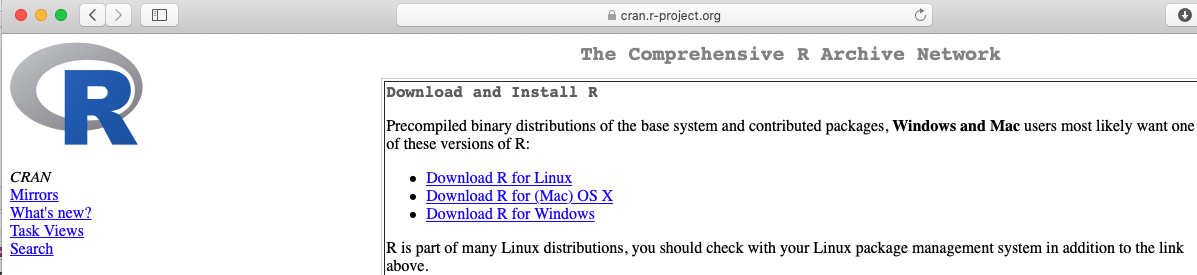
\includegraphics[width=0.85\linewidth,height=\textheight,keepaspectratio]{./images/cran.png}

\begin{itemize}
\tightlist
\item
  Select the download that matches your operating system and hardware
  (Mac OS, Windows, Linux, etc.)
\item
  You only need the ``base'' version.
\item
  Download the installer and run it. You may want to choose not to
  create shortcuts, since you will access R only through RStudio.
\end{itemize}

\subsection{Mac with Homebrew}\label{mac-with-homebrew}

\textbf{Windows and Linux users: skip this section.}

\begin{itemize}
\tightlist
\item
  If working on Mac OS and already using Homebrew to manage software
  packages, you can skip the manual download above and just run:
\end{itemize}

\begin{Shaded}
\begin{Highlighting}[]
\NormalTok{brew install r}
\end{Highlighting}
\end{Shaded}

\begin{itemize}
\tightlist
\item
  If you want to get Homebrew and install this way \textbf{on a mac},
  \href{https://www.r-bloggers.com/how-to-install-r-on-mac-ubuntu-and-windows/}{there
  are detailed instructions online} -- scroll down to ``Instructions for
  Mac Users''. Note that you don't necessarily need OpenBLAS for this
  course (as recommended on the linked website); it does not really
  matter either way.
\end{itemize}

\section{Download/Install 2 of 2:
RStudio}\label{downloadinstall-2-of-2-rstudio}

Once you have installed R, you next need to install \textbf{RStudio}.

\begin{itemize}
\tightlist
\item
  Downloads of RStudio are available at
  \url{https://rstudio.com/products/rstudio/download/}.
\item
  You should select the \textbf{free version} of \textbf{RStudio
  Desktop.}
\item
  Download and install the version that matches your operating system
\end{itemize}

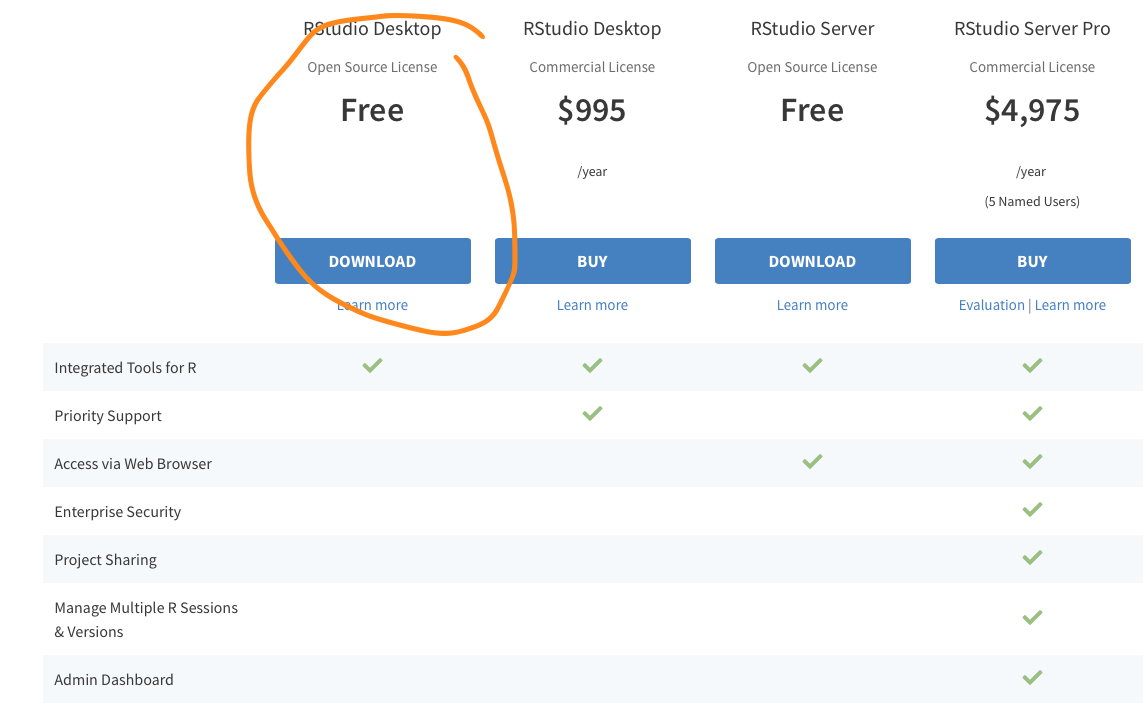
\includegraphics[width=0.85\linewidth,height=\textheight,keepaspectratio]{images/rstudio.png}

\subsection{Mac with Homebrew}\label{mac-with-homebrew-1}

\textbf{Windows and Linux users: you can't use Homebrew.}

\begin{itemize}
\tightlist
\item
  If using a mac and Homebrew, you can alternatively install RStudio
  via:
\end{itemize}

\begin{Shaded}
\begin{Highlighting}[]
\NormalTok{brew cask install rstudio}
\end{Highlighting}
\end{Shaded}

\section{Install 3/3: Packages}\label{install-33-packages}

In addition to base R and the RStudio IDE, we use a few add-on packages
that you will need to install yourself.

\begin{itemize}
\tightlist
\item
  Open RStudio
\item
  In your RStudio \textbf{Console} window, which is on the lower left by
  default, type (or copy and paste) the code below and click ``Enter''
  to run it:
\end{itemize}

\begin{Shaded}
\begin{Highlighting}[]
\FunctionTok{install.packages}\NormalTok{(}\FunctionTok{c}\NormalTok{(}\StringTok{\textquotesingle{}rmarkdown\textquotesingle{}}\NormalTok{, }\CommentTok{\# reproducible research documents}
                   \StringTok{\textquotesingle{}tidyverse\textquotesingle{}}\NormalTok{, }\StringTok{\textquotesingle{}remotes\textquotesingle{}}\NormalTok{, }\CommentTok{\# graphics and data wrangling}
                   \StringTok{\textquotesingle{}pander\textquotesingle{}}\NormalTok{, }\CommentTok{\# formatting tables}
                   \StringTok{\textquotesingle{}glmmTMB\textquotesingle{}}\NormalTok{, }\StringTok{\textquotesingle{}mgcv\textquotesingle{}}\NormalTok{, }\CommentTok{\# fitting regression models}
                   \StringTok{\textquotesingle{}car\textquotesingle{}}\NormalTok{, }\StringTok{\textquotesingle{}ggeffects\textquotesingle{}}\CommentTok{\#,  working with fitted models}
                   \CommentTok{\# optional additions:}
                   \CommentTok{\# \textquotesingle{}mosaic\textquotesingle{}, \# formula{-}based summary stats and resampling}
                   \CommentTok{\# \textquotesingle{}openintro\textquotesingle{}, \# datasets}
                   \CommentTok{\# \textquotesingle{}shiny\textquotesingle{}, \textquotesingle{}plotly\textquotesingle{}, \textquotesingle{}gganimate\textquotesingle{}, \textquotesingle{}leaflet\textquotesingle{} \# interactive graphics/maps}
\NormalTok{                   )) }
\CommentTok{\# if desired, for function to ggplot ACFs:}
\NormalTok{remotes}\SpecialCharTok{::}\FunctionTok{install\_github}\NormalTok{(}\StringTok{\textquotesingle{}stacyderuiter/s245\textquotesingle{}}\NormalTok{)}
\end{Highlighting}
\end{Shaded}

\begin{itemize}
\tightlist
\item
  In addition to the packages you listed specifically, a number of
  dependencies (other packages that the packages you requested require
  to work) will be installed.
\item
  The amount of time it takes will depend on your computer and internet
  connection speed, but as long as it finishes without any messages that
  literally say ``Error: \ldots{}'', it worked!.
\item
  If RStudio prompts you to update packages or install additional
  dependencies, it's usually a good idea to do so.
\item
  If R asks you if you want to install a certain package ``from source''
  blah, blah, ``is newer\ldots{}'' usually you can answer yes (or no)
  and it will work either way.
\item
  If you get an error or have any questions, get in touch with your
  professor.
\end{itemize}

\subsection{TeX for PDF generation}\label{tex-for-pdf-generation}

To enable generation of PDF output from Rmarkdown documents, there is a
little more code to run. (If you don't know what this means yet, you
will soon - and you \emph{do} probably need to be able to do it.)

This one has two steps: installing the package, and then \emph{using}
the package to install the PDF-generation utility.

If you already have TeX/LaTeX/MikTeX installed on your computer, you can
probably skip this installation (but it won't hurt).

\begin{Shaded}
\begin{Highlighting}[]
\FunctionTok{install.packages}\NormalTok{(}\StringTok{\textquotesingle{}tinytex\textquotesingle{}}\NormalTok{)}
\NormalTok{tinytex}\SpecialCharTok{::}\FunctionTok{install\_tinytex}\NormalTok{()  }\CommentTok{\# install TinyTeX}
\end{Highlighting}
\end{Shaded}

\subsection{Point-and-Click Option}\label{point-and-click-option}

If you would like to install the packages interactively instead of on
the command line (as already shown above), you can click the
\textbf{Packages} tab on the lower right in RStudio, then click
\emph{Install} at the top of the tab. Enter the names of the packages
you want to install in the middle ``Packages'' blank, and leave the rest
of the default options, then click ``Install''.

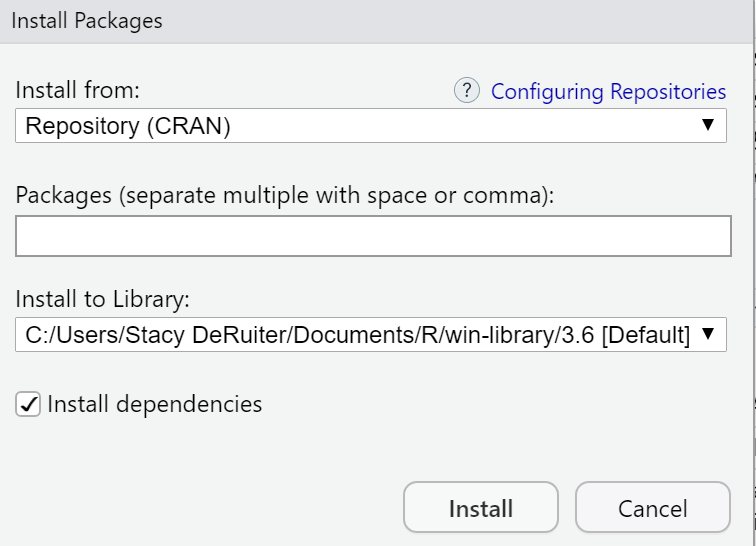
\includegraphics[width=0.85\linewidth,height=\textheight,keepaspectratio]{images/install-interactive.png}

\section{You did it!}\label{you-did-it}

If you complete all three steps above, you should have a working version
of RStudio on your machine. To use it, just open RStudio; it should look
nearly identical to the RStudio Server version you have been using
online.

You don't ever have to open or access R directly; RStudio does it all
for you.

In case of any errors or problems, contact me (stacy.deruiter at
calvin.edu) anytime and I'll do my best to help.

(Don't contact school help desks; they don't support this software).

\chapter{R Basics}\label{r-basics}

\begin{Shaded}
\begin{Highlighting}[]
\NormalTok{\#| setup: true}
\NormalTok{\#| autorun: true}
\NormalTok{\#| include: false}
\NormalTok{\#| exercise:}
\NormalTok{\#|   {-} find{-}sqrt}
\NormalTok{\#|   {-} round{-}sqrt}
\NormalTok{\#|   {-} c{-}and{-}sum}
\NormalTok{\#|   {-} name{-}a{-}variable}
\NormalTok{\#|   {-} cat{-}var}
\NormalTok{\#|   {-} check{-}out{-}data}
\NormalTok{\#|   {-} get{-}help}
\NormalTok{\#|   {-} baseball{-}mistakes}
\NormalTok{\#|   {-} look{-}at{-}MI\_lead}
\NormalTok{\#|   {-} rename{-}MI\_lead}

\NormalTok{library(readr)}
\NormalTok{library(tidyr)}
\NormalTok{library(dplyr)}
\NormalTok{library(ggformula)}
\NormalTok{library(mosaic)}
\NormalTok{library(mosaicData)}

\NormalTok{theme\_set(theme\_bw())}

\NormalTok{knitr::opts\_chunk$set(}
\NormalTok{  echo = TRUE,}
\NormalTok{  fig.align = "center",}
\NormalTok{  fig.width = 6, fig.height = 2.5)}

\NormalTok{options("readr.edition" = 1)}

\NormalTok{data(HELPrct, package = "mosaicData")}

\NormalTok{MI\_lead \textless{}{-} read\_csv(file=\textquotesingle{}https://sldr.netlify.app/data/MI\_lead.csv\textquotesingle{})}
\end{Highlighting}
\end{Shaded}

\section{Your Mission}\label{your-mission}

The purpose of this tutorial is to help you start to get familiar with
the way R works, and some basic R commands\ldots even if you haven't yet
installed R on your computer or made a
\href{https://posit.cloud}{posit.cloud} account.

This tutorial environment uses \hyperref[0]{webr}, which lets you read
some helpful information, then immediately practice writing and running
your own R code, \emph{all in your web browser}.

Here's hoping it provides a nice, gentle introduction in a controlled
environment!

\section{Communicating with R}\label{communicating-with-r}

You will do most of your work in R with \emph{code} or \emph{commands}.
Instead of pointing and clicking, you will type one or more lines of
code, which R will \emph{execute} (doing the work you have asked it to
do).

Then, R will return the results of whatever operation you asked it to do
- sometimes producing a plot, other times creating a plot.

Sometimes executing code has almost no visible effect (no plot or text
output is produced), but instead some object is created and stored in
R's \emph{environment} for later use.

\subsection{Two Key Questions}\label{two-key-questions}

To get R (or any software) to do something for you, there are two
important questions you must be able to answer. Before continuing, think
about what those questions might be.

\subsection{The Questions}\label{the-questions}

To get R (or any software) to do a job for you, there are two important
questions you must be able to answer:

\subsubsection{1. What do you want the computer to
do?}\label{what-do-you-want-the-computer-to-do}

\subsubsection{2. What must the computer know in order to do
that?}\label{what-must-the-computer-know-in-order-to-do-that}

\subsection{Providing R with the information it
needs}\label{providing-r-with-the-information-it-needs}

R \emph{functions} provide R with the answer to the first question: what
do you want the computer to do?

Most functions in R have short, but descriptive names that describe what
they do. For example, R has some functions to do basic mathematical
operations: the function \texttt{sqrt()} computes the square root of a
number, and the function \texttt{round()} rounds a number (by default,
it rounds to the nearest integer).

But just giving R a function is not enough: you also need to answer the
second question (what information does R need to do the job?). For
example, if you want to use the function \texttt{round()}, you also need
to provide R with the number you want to round!

We will provide answers to our two questions by filling in the boxes of
a basic template:

{function} ( ~information1~ , ~information2~ , \ldots)

~

(The \texttt{...} indicates that there may be some additional
\emph{input arguments} (input information we could provide to R) we
could add eventually. Some functions need only one input, but if a
function takes more than one argument, they are separated by commas.
They have names, and if named (like:
\texttt{function(input\_name\ =\ value,\ input2\_name\ =\ \textquotesingle{}value\textquotesingle{})})
they can be in any order.

\subsection{Using simple functions}\label{using-simple-functions}

Let's practice what you just learned, trying out the mathematical
\texttt{sqrt()} and \texttt{round()} functions.

Edit the code below to compute the square root of 64:

\begin{Shaded}
\begin{Highlighting}[]
\NormalTok{\#| exercise: find{-}sqrt}
\NormalTok{function(information\_R\_needs)}
\end{Highlighting}
\end{Shaded}

\begin{tcolorbox}[enhanced jigsaw, colbacktitle=quarto-callout-note-color!10!white, opacitybacktitle=0.6, titlerule=0mm, left=2mm, leftrule=.75mm, toptitle=1mm, toprule=.15mm, rightrule=.15mm, title=\textcolor{quarto-callout-note-color}{\faInfo}\hspace{0.5em}{Hint 1}, colback=white, arc=.35mm, colframe=quarto-callout-note-color-frame, bottomrule=.15mm, breakable, bottomtitle=1mm, opacityback=0, coltitle=black]

Consider using the \texttt{sqrt()} function:

\begin{Shaded}
\begin{Highlighting}[]
\FunctionTok{sqrt}\NormalTok{(\_\_\_)}
\end{Highlighting}
\end{Shaded}

\end{tcolorbox}

\begin{tcolorbox}[enhanced jigsaw, colbacktitle=quarto-callout-note-color!10!white, opacitybacktitle=0.6, titlerule=0mm, left=2mm, leftrule=.75mm, toptitle=1mm, toprule=.15mm, rightrule=.15mm, title=\textcolor{quarto-callout-note-color}{\faInfo}\hspace{0.5em}{Hint 2}, colback=white, arc=.35mm, colframe=quarto-callout-note-color-frame, bottomrule=.15mm, breakable, bottomtitle=1mm, opacityback=0, coltitle=black]

The input information that \texttt{sqrt()} needs to make your
calculation is the number you want the square root of: 64.

\end{tcolorbox}

\begin{solution}
\leavevmode

\begin{tcolorbox}[enhanced jigsaw, colbacktitle=quarto-callout-tip-color!10!white, opacitybacktitle=0.6, titlerule=0mm, left=2mm, leftrule=.75mm, toptitle=1mm, toprule=.15mm, rightrule=.15mm, title=\textcolor{quarto-callout-tip-color}{\faLightbulb}\hspace{0.5em}{Solution:}, colback=white, arc=.35mm, colframe=quarto-callout-tip-color-frame, bottomrule=.15mm, breakable, bottomtitle=1mm, opacityback=0, coltitle=black]

\begin{Shaded}
\begin{Highlighting}[]
\FunctionTok{sqrt}\NormalTok{(}\DecValTok{64}\NormalTok{)}
\end{Highlighting}
\end{Shaded}

\end{tcolorbox}

\end{solution}

Now try computing the square root of 44, \emph{and then} rounding it to
the nearest integer:

\begin{Shaded}
\begin{Highlighting}[]
\NormalTok{\#| exercise: round{-}sqrt}
\end{Highlighting}
\end{Shaded}

\begin{tcolorbox}[enhanced jigsaw, colbacktitle=quarto-callout-note-color!10!white, opacitybacktitle=0.6, titlerule=0mm, left=2mm, leftrule=.75mm, toptitle=1mm, toprule=.15mm, rightrule=.15mm, title=\textcolor{quarto-callout-note-color}{\faInfo}\hspace{0.5em}{Hint 1}, colback=white, arc=.35mm, colframe=quarto-callout-note-color-frame, bottomrule=.15mm, breakable, bottomtitle=1mm, opacityback=0, coltitle=black]

You'll need to use \emph{two} functions this time:

The \texttt{sqrt()} function, and then the \texttt{round()} function.

\begin{Shaded}
\begin{Highlighting}[]
\FunctionTok{sqrt}\NormalTok{(\_\_\_)}
\FunctionTok{round}\NormalTok{(\_\_\_)}
\end{Highlighting}
\end{Shaded}

\end{tcolorbox}

\begin{tcolorbox}[enhanced jigsaw, colbacktitle=quarto-callout-note-color!10!white, opacitybacktitle=0.6, titlerule=0mm, left=2mm, leftrule=.75mm, toptitle=1mm, toprule=.15mm, rightrule=.15mm, title=\textcolor{quarto-callout-note-color}{\faInfo}\hspace{0.5em}{Hint 2}, colback=white, arc=.35mm, colframe=quarto-callout-note-color-frame, bottomrule=.15mm, breakable, bottomtitle=1mm, opacityback=0, coltitle=black]

The input information that \texttt{sqrt()} needs to make your
calculation is the number you want the square root of: 44. Run that code
first, to get the input you will need for \texttt{round()}\ldots{}

\begin{Shaded}
\begin{Highlighting}[]
\FunctionTok{sqrt}\NormalTok{(}\DecValTok{44}\NormalTok{)}
\FunctionTok{round}\NormalTok{(\_\_\_)}
\end{Highlighting}
\end{Shaded}

\end{tcolorbox}

\begin{solution}
\leavevmode

\begin{tcolorbox}[enhanced jigsaw, colbacktitle=quarto-callout-tip-color!10!white, opacitybacktitle=0.6, titlerule=0mm, left=2mm, leftrule=.75mm, toptitle=1mm, toprule=.15mm, rightrule=.15mm, title=\textcolor{quarto-callout-tip-color}{\faLightbulb}\hspace{0.5em}{Solution:}, colback=white, arc=.35mm, colframe=quarto-callout-tip-color-frame, bottomrule=.15mm, breakable, bottomtitle=1mm, opacityback=0, coltitle=black]

\begin{Shaded}
\begin{Highlighting}[]
\FunctionTok{sqrt}\NormalTok{(}\DecValTok{44}\NormalTok{)}
\FunctionTok{round}\NormalTok{(}\FloatTok{6.63325}\NormalTok{)}
\end{Highlighting}
\end{Shaded}

Can you do it all in one go? Well\ldots yes!

\begin{Shaded}
\begin{Highlighting}[]
\FunctionTok{round}\NormalTok{(}\FunctionTok{sqrt}\NormalTok{(}\DecValTok{44}\NormalTok{))}
\end{Highlighting}
\end{Shaded}

There's also an easier-to-read way to do that, using a \emph{pipe
operator} \texttt{\textbar{}\textgreater{}}. It takes the output of one
operation and passes it as input to the next. You can read it as
\texttt{\textbar{}\textgreater{}} = ``and then\ldots{}'' so we could do:

\begin{Shaded}
\begin{Highlighting}[]
\FunctionTok{sqrt}\NormalTok{(}\DecValTok{44}\NormalTok{) }\SpecialCharTok{|\textgreater{}}
  \FunctionTok{round}\NormalTok{()}
\end{Highlighting}
\end{Shaded}

\begin{enumerate}
\def\labelenumi{\arabic{enumi}.}
\tightlist
\item
  Take the square root of 44, \emph{and then}
\item
  round the result.
\end{enumerate}

(More on pipes later!)

\end{tcolorbox}

\end{solution}

\subsection{Storing information in R:
variables}\label{storing-information-in-r-variables}

In the last section, you computed the square root of 44 and then rounded
it, perhaps like this:

\begin{Shaded}
\begin{Highlighting}[]
\FunctionTok{sqrt}\NormalTok{(}\DecValTok{44}\NormalTok{)}
\end{Highlighting}
\end{Shaded}

\begin{verbatim}
[1] 6.63325
\end{verbatim}

\begin{Shaded}
\begin{Highlighting}[]
\FunctionTok{round}\NormalTok{(}\FloatTok{6.63325}\NormalTok{)}
\end{Highlighting}
\end{Shaded}

\begin{verbatim}
[1] 7
\end{verbatim}

But to do that, you probably had to first find the root, make a note of
the result, and then provide that number to the \texttt{round} function.
What a pain!

A very useful option, if you have value (or a variable, dataset, or
other R object) that you will want to use later on, is to store it as a
named object in R. In the previous example, you might want to store the
square root of 44 in a variable called \texttt{my\_root}; then you can
provide my\_root to the \texttt{round()} function without checking the
result of the \texttt{sqrt()} calculation first:

\begin{Shaded}
\begin{Highlighting}[]
\NormalTok{my\_root }\OtherTok{\textless{}{-}} \FunctionTok{sqrt}\NormalTok{(}\DecValTok{44}\NormalTok{)}
\FunctionTok{round}\NormalTok{(my\_root)}
\end{Highlighting}
\end{Shaded}

\begin{verbatim}
[1] 7
\end{verbatim}

Notice that to assign a name to the results of some R code, you use the
symbol \texttt{\textless{}-}. You can think of it as an \emph{assignment
arrow} -- it points \emph{from} a value or item \emph{toward a name} and
assigns the name to the thing.

Try editing the code to change the name of the variable from
\texttt{my\_root} to something else, then run your new code:

\begin{Shaded}
\begin{Highlighting}[]
\NormalTok{\#| exercise: name{-}a{-}variable}
\NormalTok{my\_root \textless{}{-} sqrt(44)}
\NormalTok{round(my\_root)}
\end{Highlighting}
\end{Shaded}

\begin{tcolorbox}[enhanced jigsaw, colbacktitle=quarto-callout-note-color!10!white, opacitybacktitle=0.6, titlerule=0mm, left=2mm, leftrule=.75mm, toptitle=1mm, toprule=.15mm, rightrule=.15mm, title=\textcolor{quarto-callout-note-color}{\faInfo}\hspace{0.5em}{Hint}, colback=white, arc=.35mm, colframe=quarto-callout-note-color-frame, bottomrule=.15mm, breakable, bottomtitle=1mm, opacityback=0, coltitle=black]

Make sure you change the name \texttt{my\_root} in \emph{both} places.

\end{tcolorbox}

\begin{solution}
\leavevmode

\begin{tcolorbox}[enhanced jigsaw, colbacktitle=quarto-callout-note-color!10!white, opacitybacktitle=0.6, titlerule=0mm, left=2mm, leftrule=.75mm, toptitle=1mm, toprule=.15mm, rightrule=.15mm, title=\textcolor{quarto-callout-note-color}{\faInfo}\hspace{0.5em}{Solution}, colback=white, arc=.35mm, colframe=quarto-callout-note-color-frame, bottomrule=.15mm, breakable, bottomtitle=1mm, opacityback=0, coltitle=black]

\begin{Shaded}
\begin{Highlighting}[]
\NormalTok{your\_new\_name }\OtherTok{\textless{}{-}} \FunctionTok{sqrt}\NormalTok{(}\DecValTok{44}\NormalTok{)}
\FunctionTok{round}\NormalTok{(your\_new\_name)}
\end{Highlighting}
\end{Shaded}

\end{tcolorbox}

\end{solution}

\subsection{What if I have a list of numbers to
store?}\label{what-if-i-have-a-list-of-numbers-to-store}

Sometime you might want to create a variable that contains more than one
number. You can use the function \texttt{c()} to \emph{concatenate} a
list of numbers:

\begin{Shaded}
\begin{Highlighting}[]
\NormalTok{my\_fave\_numbers }\OtherTok{\textless{}{-}} \FunctionTok{c}\NormalTok{(}\DecValTok{4}\NormalTok{, }\DecValTok{44}\NormalTok{, }\DecValTok{16}\NormalTok{)}
\NormalTok{my\_fave\_numbers}
\end{Highlighting}
\end{Shaded}

\begin{verbatim}
[1]  4 44 16
\end{verbatim}

(First we stored the list of numbers, calling it my\_fave\_numbers; then
we printed the results to the screen by simply typing the variable name
my\_fave\_numbers).

Try making a list of your three favorite numbers, then using the
function \texttt{sum} to add them all up:

\begin{Shaded}
\begin{Highlighting}[]
\NormalTok{\#| exercise:  c{-}and{-}sum}
\end{Highlighting}
\end{Shaded}

\begin{tcolorbox}[enhanced jigsaw, colbacktitle=quarto-callout-note-color!10!white, opacitybacktitle=0.6, titlerule=0mm, left=2mm, leftrule=.75mm, toptitle=1mm, toprule=.15mm, rightrule=.15mm, title=\textcolor{quarto-callout-note-color}{\faInfo}\hspace{0.5em}{Hint}, colback=white, arc=.35mm, colframe=quarto-callout-note-color-frame, bottomrule=.15mm, breakable, bottomtitle=1mm, opacityback=0, coltitle=black]

First use \texttt{c()} to concatenate your chosen numbers (separated by
commas).

Don't forget to use \texttt{\textless{}-} to assign your list of numbers
a name!

Then, use \texttt{sum()} to add them up.

\begin{Shaded}
\begin{Highlighting}[]
\NormalTok{my\_numbers }\OtherTok{\textless{}{-}} \FunctionTok{c}\NormalTok{(\_\_\_,\_\_\_,\_\_\_)}
\FunctionTok{sum}\NormalTok{(\_\_\_)}
\end{Highlighting}
\end{Shaded}

\end{tcolorbox}

\begin{solution}
\leavevmode

\begin{tcolorbox}[enhanced jigsaw, colbacktitle=quarto-callout-note-color!10!white, opacitybacktitle=0.6, titlerule=0mm, left=2mm, leftrule=.75mm, toptitle=1mm, toprule=.15mm, rightrule=.15mm, title=\textcolor{quarto-callout-note-color}{\faInfo}\hspace{0.5em}{Solution}, colback=white, arc=.35mm, colframe=quarto-callout-note-color-frame, bottomrule=.15mm, breakable, bottomtitle=1mm, opacityback=0, coltitle=black]

This is just one possible solution.

\begin{Shaded}
\begin{Highlighting}[]
\NormalTok{my\_numbers }\OtherTok{\textless{}{-}} \FunctionTok{c}\NormalTok{(}\DecValTok{4}\NormalTok{, }\DecValTok{16}\NormalTok{, }\DecValTok{44}\NormalTok{)}
\FunctionTok{sum}\NormalTok{(my\_numbers)}
\end{Highlighting}
\end{Shaded}

Notice you \emph{could} also nest \texttt{sum()} and \texttt{c()}, or
use the pipe operator \texttt{\textbar{}\textgreater{}} to calculate the
numeric answer, \emph{but then you would not have the object
\texttt{my\_numbers} available for later use}\ldots{}

\begin{Shaded}
\begin{Highlighting}[]
\FunctionTok{sum}\NormalTok{(}\FunctionTok{c}\NormalTok{(}\DecValTok{4}\NormalTok{, }\DecValTok{16}\NormalTok{, }\DecValTok{44}\NormalTok{))}
\CommentTok{\# or }
\FunctionTok{c}\NormalTok{(}\DecValTok{4}\NormalTok{, }\DecValTok{16}\NormalTok{, }\DecValTok{44}\NormalTok{) }\SpecialCharTok{|\textgreater{}}
  \FunctionTok{sum}\NormalTok{()}
\end{Highlighting}
\end{Shaded}

\end{tcolorbox}

\end{solution}

\subsection{What about data that are not
numeric?}\label{what-about-data-that-are-not-numeric}

R can work with categorical data as well as numeric data. For example,
we could create a list of words and store it as a variable if we wanted
(feel free to try changing the words if you want):

\begin{Shaded}
\begin{Highlighting}[]
\NormalTok{\#| exercise: cat{-}var}
\NormalTok{my\_words \textless{}{-} c(\textquotesingle{}RStudio\textquotesingle{}, \textquotesingle{}is\textquotesingle{}, \textquotesingle{}awesome\textquotesingle{})}
\NormalTok{my\_words}
\end{Highlighting}
\end{Shaded}

\subsection{What if I have a LOT more data to
store?}\label{what-if-i-have-a-lot-more-data-to-store}

\texttt{c()} works great for creating small lists of just a few values,
but it is \emph{not} a good way to enter or store large data tables -
there is lots of potential for user error. In this course, you will
usually be given a dataset already in electronic form; if you need to
create one, you would turn to spreadsheet or database software. Either
way you read the existing data file into R directly.

In R, these larger datasets are stored as objects called
\texttt{data.frame}s. The next sections will get you started using them.

\section{How should data tables be organized for statistical
analysis?}\label{how-should-data-tables-be-organized-for-statistical-analysis}

A comprehensive guide to good practices for formatting data tables is
available at \url{http://kbroman.org/dataorg/}.

A few key points to keep in mind:

\begin{itemize}
\tightlist
\item
  This data table is for the computer to read, not for humans! So
  eliminate formatting designed to make it ``pretty'' (color coding,
  shading, fonts\ldots)
\item
  Use short, simple variable names that do not contain any spaces or
  special characters (like ?, \$, \%, -, etc.)
\item
  Organize the table so there is one column for every variable, and one
  row for every observation (person/place/thing for which data were
  collected).
\item
  Use informative variable values rather than arbitrary numeric codes.
  For example, a variable Color should have values `red', `white', and
  `blue' rather than 1, 2, and 3.
\end{itemize}

You will have chances to practice making your own data files and
importing them into R outside this tutorial.

\section{Using built-in datasets in
R}\label{using-built-in-datasets-in-r}

R has a number of built-in datasets that are accessible to you as soon
as you start RStudio.

In addition to the datasets that are included with base R, there are
add-on \emph{packages} for R that contain additional software tools and
sometimes datasets.

To use datasets contained in a package, you have to load the package by
running the command:

\begin{Shaded}
\begin{Highlighting}[]
\FunctionTok{library}\NormalTok{(packagename) }
\end{Highlighting}
\end{Shaded}

\subsection{Example of loading a
package}\label{example-of-loading-a-package}

For example, we will practice looking at a dataset from the package
\texttt{mosaic}.

Before we can access the data, we have to load the package. The code
might look like this:

\begin{Shaded}
\begin{Highlighting}[]
\FunctionTok{library}\NormalTok{(mosaic)}
\end{Highlighting}
\end{Shaded}

\textbf{(Nothing obvious will happen when you run this code\ldots it
basically just gives R permission to access the package, so there is
often no output visible.)}

\subsection{Viewing a dataset}\label{viewing-a-dataset}

The \texttt{mosaic} package includes a dataset called \texttt{HELPrct}.

If you just run the dataset name (\texttt{HELPrct}) as a command, R will
print some (or all - egad!) of the dataset out to the screen! (So
don't\ldots)

\textbf{But}\ldots how can we extract selected, useful information about
a dataset?

\subsection{Gathering information about a
dataset}\label{gathering-information-about-a-dataset}

There are a few functions that make it easier to take a quick look at a
dataset:

\begin{itemize}
\tightlist
\item
  \texttt{head()} prints out the first few rows of the dataset.
\item
  \texttt{names()} prints out the names of the variables (columns) in
  the dataset
\item
  \texttt{dplyr::glimpse()} (function \texttt{glimpse()} from package
  \texttt{dplyr}) gives an short list-like overview of the dataset
\item
  \texttt{skimr::skim()} (function \texttt{skim()} from the package
  \texttt{skimr}) prints out more detailed graphical summary information
  about a dataset
\item
  \texttt{nrow()} reports the number of rows (observations or cases) in
  the dataset
\item
  \texttt{ncol()} reports the number of columns (variables) in the
  dataset
\end{itemize}

Try applying each of these functions to the \texttt{HELPrct} data and
see what the output looks like each time:

\begin{Shaded}
\begin{Highlighting}[]
\NormalTok{\#| exercise: check{-}out{-}data}
\NormalTok{function(\_\_\_\_)}
\end{Highlighting}
\end{Shaded}

\begin{solution}
\leavevmode

\begin{tcolorbox}[enhanced jigsaw, colbacktitle=quarto-callout-note-color!10!white, opacitybacktitle=0.6, titlerule=0mm, left=2mm, leftrule=.75mm, toptitle=1mm, toprule=.15mm, rightrule=.15mm, title=\textcolor{quarto-callout-note-color}{\faInfo}\hspace{0.5em}{Solution}, colback=white, arc=.35mm, colframe=quarto-callout-note-color-frame, bottomrule=.15mm, breakable, bottomtitle=1mm, opacityback=0, coltitle=black]

The input for each of the functions is the name of the dataset:
\texttt{HELPrct}.

\begin{Shaded}
\begin{Highlighting}[]
\FunctionTok{head}\NormalTok{(HELPrct)}
\FunctionTok{names}\NormalTok{(HELPrct)}
\FunctionTok{nrow}\NormalTok{(HELPrct)}
\FunctionTok{ncol}\NormalTok{(HELPrct)}
\NormalTok{skimr}\SpecialCharTok{::}\FunctionTok{skim}\NormalTok{(HELPrct)}
\NormalTok{dplyr}\SpecialCharTok{::}\FunctionTok{glimpse}\NormalTok{(HELPrct)}
\end{Highlighting}
\end{Shaded}

In this case, the point is usually to view the information on-screen,
not to store it for later use, so we have not used \texttt{\textless{}-}
at all to store any output for later use or reference.

\end{tcolorbox}

\end{solution}

\subsection{Getting more help}\label{getting-more-help}

You can get help related to R function, and built-in R datasets, using a
special function: \texttt{?}. Just type ? followed by the name of the
function or dataset you want help on:

\begin{Shaded}
\begin{Highlighting}[]
\NormalTok{\#| exercise: get{-}help}
\end{Highlighting}
\end{Shaded}

\begin{solution}
\leavevmode

\begin{tcolorbox}[enhanced jigsaw, colbacktitle=quarto-callout-note-color!10!white, opacitybacktitle=0.6, titlerule=0mm, left=2mm, leftrule=.75mm, toptitle=1mm, toprule=.15mm, rightrule=.15mm, title=\textcolor{quarto-callout-note-color}{\faInfo}\hspace{0.5em}{Solution}, colback=white, arc=.35mm, colframe=quarto-callout-note-color-frame, bottomrule=.15mm, breakable, bottomtitle=1mm, opacityback=0, coltitle=black]

For example, if you want to know about the function \texttt{nrow()}:

\begin{Shaded}
\begin{Highlighting}[]
\NormalTok{?nrow}
\end{Highlighting}
\end{Shaded}

\end{tcolorbox}

\end{solution}

\section{Reading in data from a file}\label{reading-in-data-from-a-file}

For this class, you will often be asked to analyze data that is stored
in files that are available online - usually in csv format. It's simple
to read them into R. For example, we can read in the file MI\_lead.csv,
which is stored at \url{https://sldr.netlify.app/data/MI_lead.csv} using
the function \texttt{read\_csv()} (from package \texttt{readr} or
super-package \texttt{tidyverse}):

\begin{Shaded}
\begin{Highlighting}[]
\FunctionTok{library}\NormalTok{(readr) }\CommentTok{\# the readr package contains the read\_csv() function}
\NormalTok{MI\_lead }\OtherTok{\textless{}{-}} \FunctionTok{read\_csv}\NormalTok{(}\AttributeTok{file =} \StringTok{\textquotesingle{}https://sldr.netlify.app/data/MI\_lead.csv\textquotesingle{}}\NormalTok{)}
\end{Highlighting}
\end{Shaded}

\subsection{The most common mistakes}\label{the-most-common-mistakes}

The code below contains several of the \textbf{most common mistakes}
students make when they try to read in a data file. See if you can find
and correct them \textbf{all}!

The code below - if corrected - \emph{would} (on posit.cloud or in
standalone R/RStudio) run without an error and read in some baseball
statistics from the file
\url{http://stacyderuiter.github.io/teachingdata/data-raw/baseball.csv}.

Here in this tutorial, it may give the error:
\texttt{!\ curl\ package\ not\ installed,\ falling\ back\ to\ using\ url()}
-- there's not a straightforward fix, sorry, but try it on the server if
you want to prove to yourself that it works!

\begin{Shaded}
\begin{Highlighting}[]
\NormalTok{\#| exercise: baseball{-}mistakes}
\NormalTok{read\_csv(http://stacyderuiter.github.io/teachingdata/data{-}raw/base)}
\end{Highlighting}
\end{Shaded}

\begin{tcolorbox}[enhanced jigsaw, colbacktitle=quarto-callout-note-color!10!white, opacitybacktitle=0.6, titlerule=0mm, left=2mm, leftrule=.75mm, toptitle=1mm, toprule=.15mm, rightrule=.15mm, title=\textcolor{quarto-callout-note-color}{\faInfo}\hspace{0.5em}{Hints}, colback=white, arc=.35mm, colframe=quarto-callout-note-color-frame, bottomrule=.15mm, breakable, bottomtitle=1mm, opacityback=0, coltitle=black]

Think about:

\begin{itemize}
\tightlist
\item
  Is the filename or URL spelled correctly, with no typos?
\item
  Is the filename or URL in quotation marks (either '' or ' work
  equally)?
\item
  Is the URL complete (including the file extension ``.csv'')
\item
  Was \texttt{\textless{}-} used to assign a \emph{name} to the dataset
  once read in? (Otherwise it will just be uselessly printed to the
  screen and not available for later use!)
\end{itemize}

\end{tcolorbox}

\begin{solution}
\leavevmode

\begin{tcolorbox}[enhanced jigsaw, colbacktitle=quarto-callout-note-color!10!white, opacitybacktitle=0.6, titlerule=0mm, left=2mm, leftrule=.75mm, toptitle=1mm, toprule=.15mm, rightrule=.15mm, title=\textcolor{quarto-callout-note-color}{\faInfo}\hspace{0.5em}{Solution}, colback=white, arc=.35mm, colframe=quarto-callout-note-color-frame, bottomrule=.15mm, breakable, bottomtitle=1mm, opacityback=0, coltitle=black]

\begin{Shaded}
\begin{Highlighting}[]
\NormalTok{baseball\_data }\OtherTok{\textless{}{-}} \FunctionTok{read\_csv}\NormalTok{(}\AttributeTok{file =} \StringTok{\textquotesingle{}http://stacyderuiter.github.io/teachingdata/data{-}raw/baseball.csv\textquotesingle{}}\NormalTok{)}
\end{Highlighting}
\end{Shaded}

\end{tcolorbox}

\end{solution}

\subsection{What about local files?}\label{what-about-local-files}

The same function, \texttt{read\_csv()}, can be used to read in a local
file. You just need to change the input to \texttt{read\_csv()} --
instead of a URL, you provide a path and filename (in quotes). For
example, the input
\texttt{file\ =\ \textquotesingle{}https://sldr.netlify.app/data/MI\_lead.csv\textquotesingle{}}
might become
\texttt{file\ =\ \textquotesingle{}C:\textbackslash{}\textbackslash{}Data\textbackslash{}\textbackslash{}MI\_lead.csv\textquotesingle{}}.

We won't do an example in this tutorial because it's not straightforward
to work with local files within a tutorial environment, but you can
practice it once you are working independently in RStudio.

If you are working on the server r.cs.calvin.edu, you will have to
\emph{upload} files to your cloud space on the server before you can
read them in (RStudio on the server cannot access files on your
computer's hard drive). Look in the ``Files'' tab on the lower right,
and then click ``Upload.''

\subsection{Named input arguments}\label{named-input-arguments}

The input argument we provided to R is the URL (in quotes -- either
single or double quotes are fine). But notice that this time, we gave
the input argument a \emph{name}, ``file'', and specified its value with
an equal sign.

This is not \emph{required} - the command works fine without it:

\begin{Shaded}
\begin{Highlighting}[]
\NormalTok{MI\_lead }\OtherTok{\textless{}{-}} \FunctionTok{read\_csv}\NormalTok{(}\StringTok{\textquotesingle{}https://sldr.netlify.app/data/MI\_lead.csv\textquotesingle{}}\NormalTok{)}
\end{Highlighting}
\end{Shaded}

However, if a function has \emph{more than just one} input argument,
it's good to get in the habit of providing names for the inputs. If you
provide names, then the order in which you list the inputs doesn't
matter; without names, \textbf{the order matters} and you have to use ?
to figure out what order R expects!

\subsection{Renaming variables in a
dataset}\label{renaming-variables-in-a-dataset}

This is an advanced topic, so don't worry if it seems complicated; for
now, it just nice to realize some of the power R has to clean up and
reorganize data.

What if we didn't like the names of the \texttt{MI\_lead} variables? For
example, a new user of the dataset might not know that that ELL stands
for ``elevated lead levels'' and that ELL2005 gives the
\emph{proportion} of tested kids who had elevated lead levels in the
year 2005.

If we wanted to use a clearer (though longer) variable name, we might
prefer ``prop\_elevated\_lead\_2005'' instead of ``ELL2005'' -- more
letters to type, but a bit easier to understand for a new user. How can
we tell R we want to rename a variable?

We use the code:

\begin{Shaded}
\begin{Highlighting}[]
\NormalTok{MI\_lead }\OtherTok{\textless{}{-}}\NormalTok{ MI\_lead }\SpecialCharTok{|\textgreater{}}
  \FunctionTok{rename}\NormalTok{(}\AttributeTok{prop\_elevated\_lead\_2005 =}\NormalTok{ ELL2005)}

\FunctionTok{glimpse}\NormalTok{(MI\_lead)}
\end{Highlighting}
\end{Shaded}

The code above uses some tools you've seen, and some more advanced ones
you haven't seen yet. The symbol \texttt{\textbar{}\textgreater{}} is
called a ``pipe'' and basically means ``and then\ldots{}'' Translated
into words, the code above tells R:

\begin{itemize}
\tightlist
\item
  Make a dataset called \texttt{MI\_lead} by starting with the dataset
  \texttt{MI\_lead}.
\item
  \textbf{Next, take the results do something more with them}
  (\texttt{\textbar{}\textgreater{}}) \ldots{}
\item
  \texttt{rename()} a variable. What I want to rename is the variable
  \texttt{ELL2005}. Its new name should be
  \texttt{prop\_elevated\_lead\_2005}.''
\end{itemize}

\emph{See\ldots you can already start to make sense of even some pretty
complicated (and useful) code.}

Note: If you give R several commands, \emph{not} connected by pipes, it
will do the first, then the second, then the third, and so on. R doesn't
need the pipe for permission to continue! Instead, the pipe tells R to
take the \emph{results} from the first command, and use them as the
input or starting material for the next command.

\subsection{Check out the data}\label{check-out-the-data}

OK, back to business - simple functions and datasets in R.

It's your turn to practice now. Use one of the functions you have
learned so far to extract some information about the MI\_lead dataset.

How many rows are in the dataset? How many variables (columns)?

What are the variables named, and what are their values like?

\emph{Remember, \texttt{?} won't work on MI\_lead because it's not a
built-in R dataset. Also, the dataset MI\_lead is already read in for
you, here\ldots so you don't need to use \texttt{read\_csv()}.}

\begin{Shaded}
\begin{Highlighting}[]
\NormalTok{\#| exercise: look{-}at{-}MI\_lead}
\end{Highlighting}
\end{Shaded}

\section{Review}\label{review}

What have you learned so far? More than you think!

\subsection{Functions in R}\label{functions-in-r}

You've learned that R code is made up of functions, which are generally
named descriptively according to the job they do. Functions have one or
more input arguments, which is where you provide R with all the data and
information it needs to do the job. The syntax for calling a function
uses the template:

{function} ( ~information1~ , ~information2~ , \ldots)

~

\subsection{Variables in R}\label{variables-in-r}

You've practiced creating variables in R using \texttt{c()}, and saving
information (or the results of a computation) using the assignment arrow
\textless-.

\subsection{Datasets in R}\label{datasets-in-r}

You've considered several different ways to get datasets to work with in
R: you can use datasets that are built in to R or R packages, or you can
use \texttt{read\_csv()} to read in data files stored in .csv format.

\subsection{Vocabulary}\label{vocabulary}

You should now be able to define and work with some R-related terms:

\begin{itemize}
\tightlist
\item
  \emph{code} or \emph{commands} that R can \emph{execute}
\item
  \emph{function} and \emph{inputs} or \emph{arguments}
\item
  \emph{assignment arrow}: \texttt{\textless{}-}
\item
  \emph{pipe} = ``and then\ldots{}'': \texttt{\textbar{}\textgreater{}}
  (note: \texttt{\textbar{}\textgreater{}} is an older way of writing a
  pipe, and it does basically the \emph{same} thing as
  \texttt{\textbar{}\textgreater{}})
\end{itemize}

\section{Congratulations!}\label{congratulations}

You just completed your first tutorial on R, and wrote some of your own
R code. I \emph{knew} you could do it\ldots{}

Want more help and practice? Consider checking out outside resources
from posit: \url{https://posit.cloud/learn/primers}

\chapter{Using Quarto}\label{using-quarto}

\section{Instructions}\label{instructions}

While you work through this chapter, you will create a Quarto (.qmd)
document.

Quarto lets you combine R code, output, and text in a single document
that can be rendered in HTML, PDF, Word and more formats.

It's like magic: you save all your text and R code in a simple file;
when you're ready, push a button and it's compiled into an output
document with nicely formatted text, code (optional to include, but for
this class you always will), and \textbf{all the figures and tables
generated by your code}.

Since all the data analysis and results are automatically included in
the compiled output document, your work is \emph{reproducible} and it's
easy to re-do analysis if the data change, or if a mistake is uncovered.

\section{Reference Materials}\label{reference-materials}

For more details on using Quarto, and detailed documentation, see
\url{https://Quarto.org/docs/guide/}.

Quarto and posit also provide substantial resources for learners. This
tutorial is tailored to our course, including just the stuff you need
and not much you won't use frequently. But if you want \emph{even more}
about Quarto, you might check out:

\begin{itemize}
\tightlist
\item
  Tutorials for beginners at
  \url{https://Quarto.org/docs/get-started/hello/rstudio.html}
  (\href{https://Quarto.org/docs/get-started/hello/rstudio.html}{Hello,
  Quarto!} and
  \href{https://Quarto.org/docs/get-started/computations/rstudio.html}{Computations}
  are most relevant.)
\item
  Detailed documentation at \url{https://Quarto.org/docs/guide/}.
\end{itemize}

\subsection{\texorpdfstring{\emph{Optional}
Video}{Optional Video}}\label{optional-video}

If you love video introductions, consider also this
\href{https://youtu.be/_f3latmOhew}{23-minute offering from posit and
Mine Cetinkaya-Rundel}:

\section{Logistics}\label{logistics}

To create a .qmd file, you will have to work in RStudio (outside this
tutorial environment). So, as you work on this tutorial, you will
probably switch back and forth between the tutorial itself and an
RStudio session on your computer or on the server at
\url{https://r.stem.calvin.edu} (or if not at Calvin, at
\href{https://posit.cloud}{posit.cloud}).

\emph{Historical Note: The precursor of the Quarto document is the
Rmarkdown (.rmd) document (and even older - the Sweave document). If you
know and love one of those, you may use it, but probably best to upgrade
to Quarto, which is superceding them.}

\section{Getting Started}\label{getting-started-1}

\subsection{Logging in to RStudio}\label{logging-in-to-rstudio}

Log in to your account at \url{https://r.stem.calvin.edu} (or if not at
Calvin, at \href{https://posit.cloud}{posit.cloud}).

Or, if you installed R on your own machine, open RStudio.

\subsection{Panels}\label{panels}

When you open RStudio, you will see at least three different panels: The
\emph{Console} is on the left. On the upper right are
\emph{Environment}, \emph{History} and maybe more; on the lower right
are \emph{Files}, \emph{Plots}, and \emph{Packages}. Explore a little to
try to see what is there!

\emph{Files} shows you the files saved in your personal space on the
server. You can organize, upload, and delete files and folders.

\subsection{Executing code in R}\label{executing-code-in-r}

You can \emph{do} things in R by typing commands in the \emph{Console}
panel.

\textbf{However, working that way makes it hard to keep a record of your
work (and hard to redo things if anything changes or if a mistake was
made)}.

For this class, you will instead \textbf{work in Quarto files, which can
contain text, R code, and R output (such as figures)}.

After you have opened a file (like an RMarkdown file) on the RStudio
server, the \emph{Console} panel will be on the lower left and the newly
opened file will be on the top left. Let's learn how to do it\ldots{}

\section{Quarto (qmd) Files}\label{quarto-qmd-files}

\subsection{Quarto files are
stand-alone!}\label{quarto-files-are-stand-alone}

Every Quarto file (qmd file) must be completely stand-alone. It doesn't
share any information with the \emph{Console} or the \emph{Environment}
that you see in your RStudio session. \textbf{All} R code that you need
to do whatever you are trying to do must be included in the qmd file
itself!

For example, if you use the point-and-click user interface in the
RStudio \emph{Environment} tab to import a data file, that dataset will
\emph{not} be available when rendering your qmd file.

Similarly, if you load the \texttt{mosaic} package by typing in the
\emph{Console} window,

\begin{Shaded}
\begin{Highlighting}[]
\FunctionTok{library}\NormalTok{(mosaic)}
\end{Highlighting}
\end{Shaded}

\textbf{\texttt{mosaic} functions and data will not be available to use
within the qmd file.}

\begin{quote}
\begin{quote}
So: Keep your qmd files stand-alone! (You have no choice,
actually\ldots)
\end{quote}
\end{quote}

\subsection{Create a Quarto file}\label{create-a-quarto-file}

In RStudio, navigate to File -\textgreater{} New File -\textgreater{}
Quarto Document\ldots, or click on the white rectangle with a green
circle+ :

\begin{center}
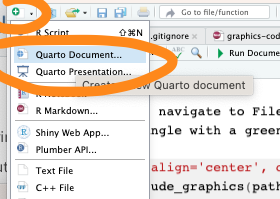
\includegraphics[width=0.85\linewidth,height=\textheight,keepaspectratio]{images/new-quarto-document.png}
\end{center}

and select Quarto from the drop-down menu.

\textbf{Choose html or pdf output.}

(\emph{Why not Word? Too much temptation to make changes and do
formatting after the fact in Word\ldots which makes your work
no-longer-reproducible. In qmd, you have documented everything you've
done. If you make changes after rendering to Word, that's not true
anymore.})

\subsection{Save your qmd file}\label{save-your-qmd-file}

Save your file by clicking on the disk icon at the top of the file tab
(give it a clear file name like deruiter\_quarto\_practice.qmd).

Do your best to avoid spaces and special characters in your file names.

\textbf{If on a server, the file will be saved to the cloud, not to your
computer.}

All your files will be accessible in the RStudio \emph{Files} tab (lower
right panel) whenever you log into RStudio, regardless of which computer
you are using. You may organize them into directories (folders) if you
want.

\begin{center}
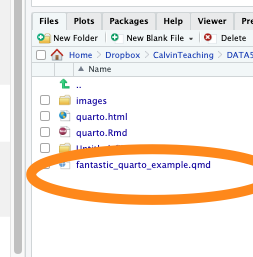
\includegraphics[width=0.85\linewidth,height=\textheight,keepaspectratio]{images/qmd-in-file-pane.png}
\end{center}

\subsection{Render!}\label{render}

How do qmd files actually work? What's so cool about them?

Click on the \emph{fat blue arrow} next to the word ``Render'' at the
top of the file window.

\begin{center}

\includegraphics[width=0.85\linewidth,height=\textheight,keepaspectratio]{images/render.png}
\end{center}

Check out the rendered html or pdf result, and compare it to the
original Quarto file.

Wow!

\subsection{Source vs.~Visual Editor}\label{source-vs.-visual-editor}

Look to the upper right corner of your qmd file. You should see some
buttons that allow you to toggle between ``Source'' and ``Visual''
editor modes.

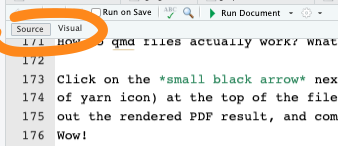
\includegraphics[width=0.6\linewidth,height=\textheight,keepaspectratio]{images/source-visual.png}

In your own file, toggle back and forth a few times. The \textbf{Source}
mode lets you see (and type) the straight-up markdown -- which is
probably nice if you're already used to it, and annoying or mystifying
if not. The \textbf{Visual} mode is more of a
what-you-see-is-what-you-get (like the rendered version),
point-and-click type interface. You may use whichever you prefer.

Be aware that if you are going to copy/paste between documents, you
probably want to do so in \textbf{Source} mode.

\subsection{Personalize your Markdown
file}\label{personalize-your-markdown-file}

At the top of the Quarto file, there is a section called the ``YAML
header''. It starts and ends with 3 dashes - - -.

\begin{quote}
\begin{quote}
In this part of the file, be very careful what you type: a stray space
or character will lead to an error.
\end{quote}
\end{quote}

This is where you can enter an appropriate title, author(s), and date
(within the quotation marks). You can also choose the format you want to
render to (usually pdf or html -- not in quotes).

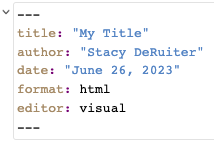
\includegraphics[width=0.4\linewidth,height=\textheight,keepaspectratio]{images/yaml.png}

Customize your YAML header in your own Quarto doc, and then render again
to see the effect.

Make sure you do this for every assignment! (No prof or boss likes
getting submissions called ``Untitled''\ldots)

\section{Quarto YAML settings}\label{quarto-yaml-settings}

\subsection{PDF or html?}\label{pdf-or-html}

For our course, you can choose to render to \emph{either} an html file
or a PDF file.

So, you'll have either \texttt{format:\ pdf} or \texttt{format:\ html}
in your YAML header. You can also try \texttt{format:\ typst} to render
PDF files a bit faster (learn more about
\href{https://quarto.org/docs/output-formats/typst.html}{typst output
format} online).

But \emph{if} you choose html, there's an important change you have to
make to the YAML header to ensure your html file is stand-alone.
Meaning: you want all images, etc. to be embedded in the one file rather
than stored in an accompanying folder. Otherwise, when you (say) upload
the file on Moodle or email it, all the images and graphs will be
omitted\ldots yikes! Yes, embedding these makes the file larger, but if
you are sharing the rendered html document, you need to.

\textbf{If rendering to html, it is} \emph{essential} \textbf{that you
specify the setting \texttt{embed-resources:\ true}!}

So, \emph{make sure} you add \texttt{embed-resources:\ true} after the
entry \texttt{format:\ html:} in your YAML header, exactly as shown
below.

Make sure to keep the spacing and line breaks just as shown.

The indents are each two spaces, so there are 2 spaces before
\texttt{html:} and 4 before \texttt{embed-resources:}.

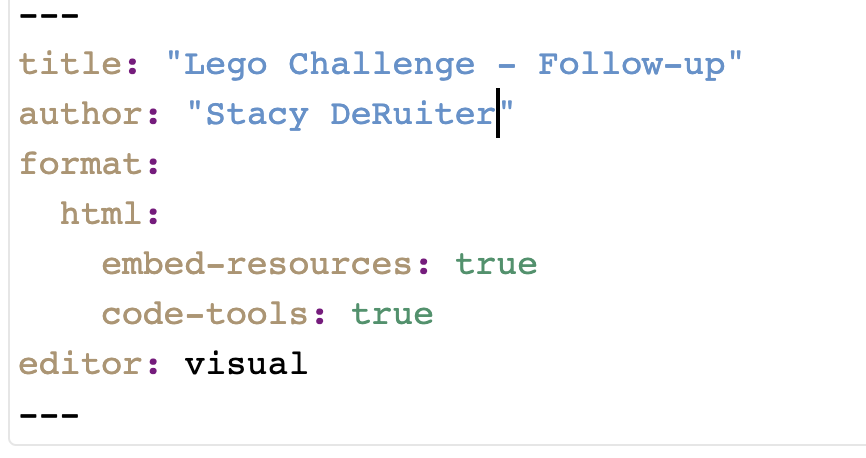
\includegraphics[width=0.75\linewidth,height=\textheight,keepaspectratio]{images/embed.png}

\subsection{Code tools}\label{code-tools}

Note that the YAML header shown above also had a second option activated
for rendered html files: \texttt{code-tools:\ true}.

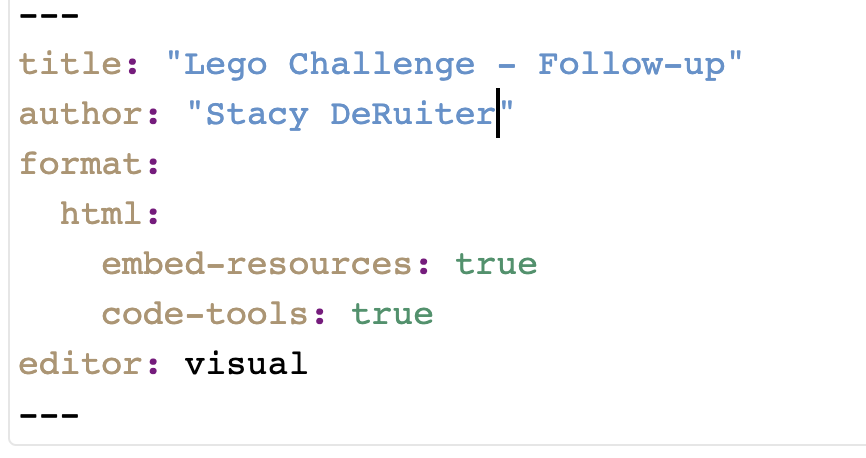
\includegraphics[width=0.75\linewidth,height=\textheight,keepaspectratio]{images/embed.png}

What does this one do?

It adds a button ``Code'' at the top right of your file.

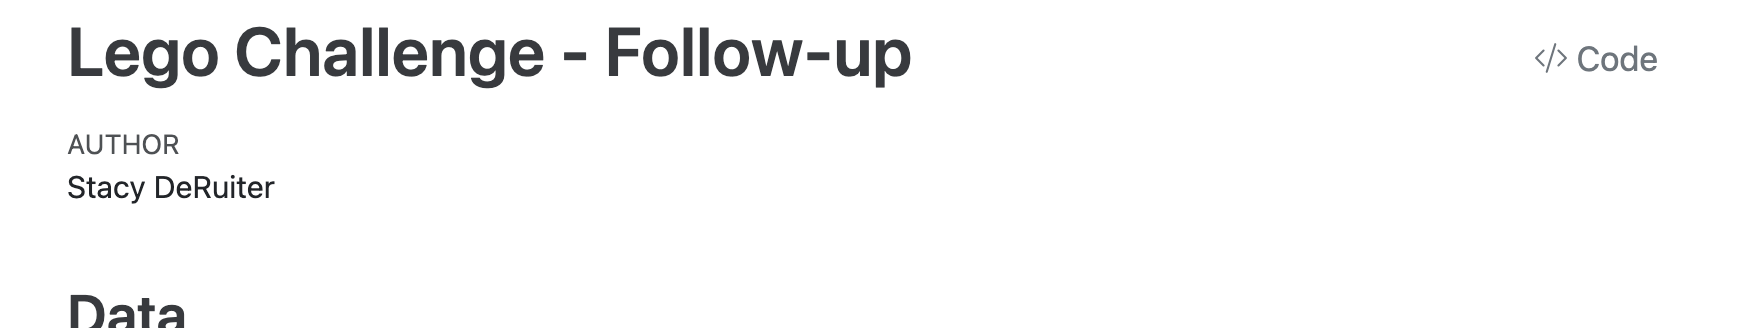
\includegraphics[width=0.75\linewidth,height=\textheight,keepaspectratio]{images/code-tools-button.png}

If you click it, you can view and copy the source code (basically, the
contents of the original qmd file before rendering). This is not a bad
option, for example for homework, as it allows me to see every detail of
the settings you used and may help me troubleshoot any issues.

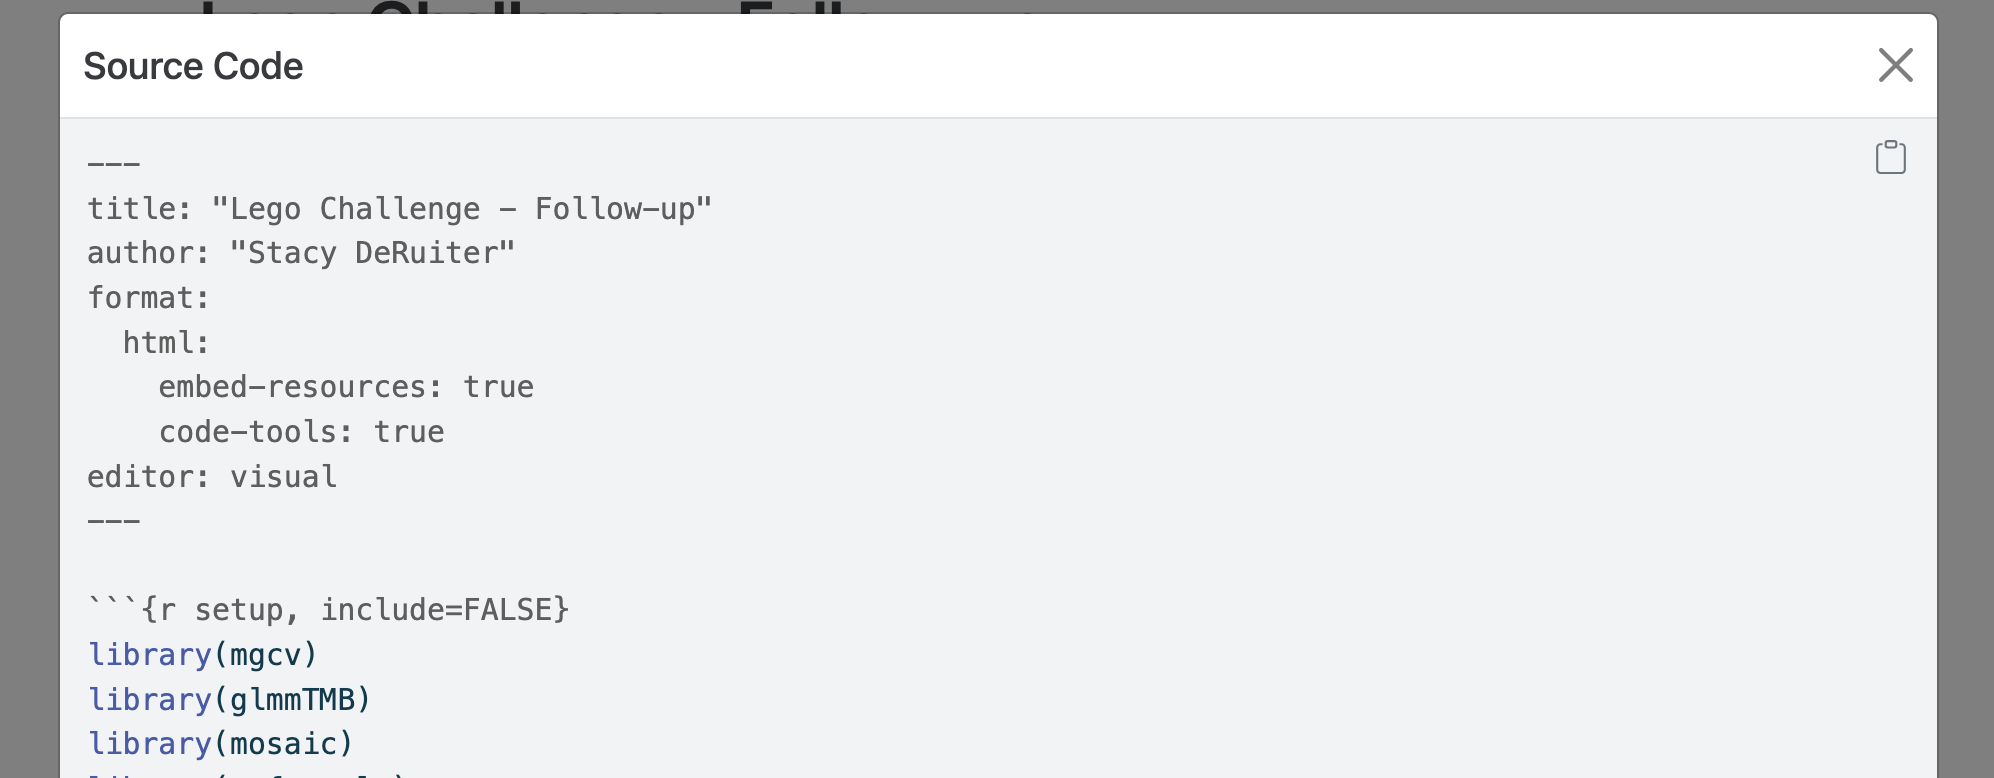
\includegraphics[width=0.75\linewidth,height=\textheight,keepaspectratio]{images/code-tools-copy.png}

\section{Text and Code in Quarto}\label{text-and-code-in-quarto}

\subsection{Text}\label{text}

The Quarto file is where you save all the R commands you want to use,
plus any text commenting on the work you are doing and the results you
get. Parts of the file with a plain white background are normal text.

You can format the text. For example, enclosing a word in asterisks will
generate italics, so *my text* in the qmd file will become \emph{my
text} in the PDF. Using two asterisks instead of one will generate
boldface, so **my text** becomes \textbf{my text}. You can also make
bulleted lists, numbered lists, section headers, and more. For example,

\#\#\#\# Some Text

becomes

\subsubsection{Some Text}\label{some-text}

(a sub-section header). Fewer hashtags make the text even larger, and
more make it smaller.

Caution! Forgetting the space after the last hashtag will format your
text verbatim rather than as a header (\#fail). Failing to leave a blank
line before the header can also make formatting fail.

Check out the Quarto Markdown Basics reference at
\url{https://quarto.org/docs/authoring/markdown-basics.html} for more
examples of how to format text in Quarto.

Before moving on, try a few of the tricks you just learned in your qmd
file. Make it pretty!

\subsection{qmd file anatomy: R code
chunks}\label{qmd-file-anatomy-r-code-chunks}

An qmd file can (of course!) contain one or more \textbf{R code chunks.}
These sections of the file have a grey background onscreen. In Source
mode, each one begins with

```\{r\}

and ends with

```

like so:

\begin{center}
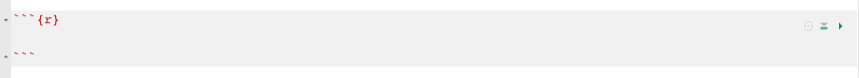
\includegraphics[width=0.85\linewidth,height=\textheight,keepaspectratio]{images/r-chunk-source.png}
\end{center}

In Visual mode you can't see the `:

\begin{center}
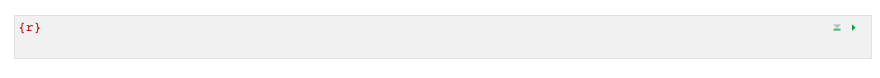
\includegraphics[width=0.85\linewidth,height=\textheight,keepaspectratio]{images/r-chunk-visual.png}
\end{center}

\subsection{How to add a new R code chunk to your
file}\label{how-to-add-a-new-r-code-chunk-to-your-file}

To add a code chunk to your file in Source editor mode, you have three
options.

\begin{enumerate}
\def\labelenumi{\arabic{enumi}.}
\tightlist
\item
  You can type in the header and footer by hand to start and end the
  chunk.
\item
  You can click on the ``add chunk'' button at the top right. It's a
  green box with the C inside (at the top of the qmd file; choose the
  first option, ``R'', in the pulldown) to insert an empty chunk.
\item
  You can use a keyboard shortcut: Windows, Ctrl + Alt + I or OS X, Cmd
  + Option + I
\end{enumerate}

When you click the \textbf{Render} button, code in code chunks will be
run, and any output will be included in the document.

\begin{center}
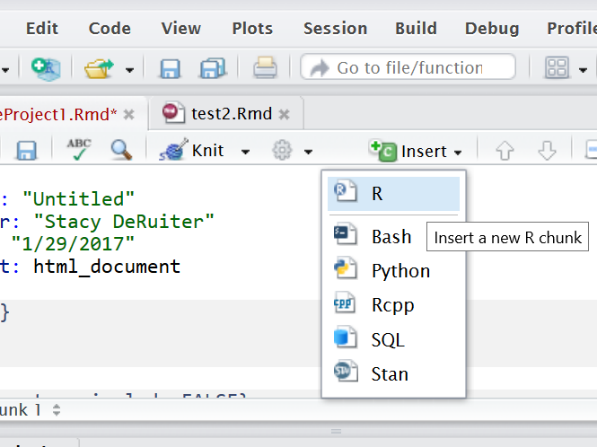
\includegraphics[width=0.85\linewidth,height=\textheight,keepaspectratio]{images/InsertCodeChunk.png}
\end{center}

\subsection{Setup Chunk}\label{setup-chunk}

Consider using the first R code chunk in a qmd file to specify settings
(for graphics, display, etc.). In this chunk, you can also give R
permission to use certain packages (software toolkits) with

\begin{Shaded}
\begin{Highlighting}[]
\FunctionTok{library}\NormalTok{(packagename) }
\end{Highlighting}
\end{Shaded}

For example, we will use the \texttt{ggformula} package for graphics.
So, verify that the first R code chunk in your file includes the line
\texttt{library(ggformula)}.

You can also specify options for each R code chunk - these go at the
top, prefaced by \texttt{\#\textbar{}}. A typical setup chunk for our
course might look like:

\begin{center}
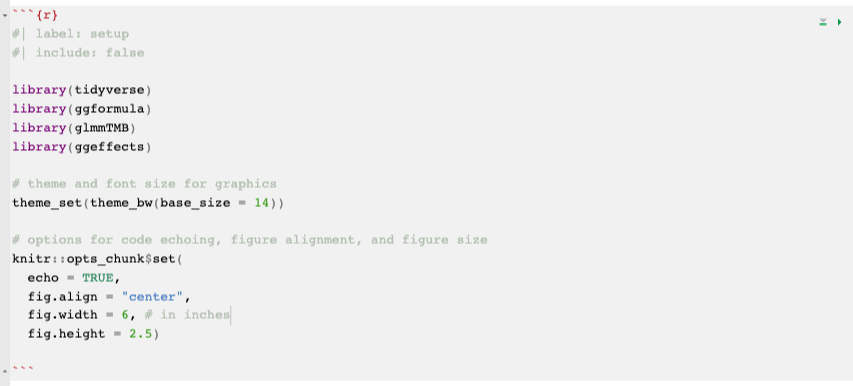
\includegraphics[width=0.85\linewidth,height=\textheight,keepaspectratio]{images/setup-chunk.png}
\end{center}

Notice that several packages are loaded (that we will use frequently).
\texttt{theme\_set()} is used to specify some settings for graph output,
and \texttt{knitr::opts\_chunk\$set()} is used to specify whether or not
to include R code in the rendered file (Yes please: use
\texttt{echo:\ true}!) and specify the default figure size.

There are \emph{tons} more options and settings, and you can explore
them at \url{https://yihui.org/renderr/options/\#chunk-options}.

But for now, if you use something like the setup chunk shown above, it
should work well and have what you need for almost all work in this
course.

\subsection{The settings chunk is
invisible!}\label{the-settings-chunk-is-invisible}

If you look carefully at the rendered output, you will see that the
setup chunk does \emph{not} appear there. That's intentional - when you
load packages with \texttt{library()}, they often print a lot of long
and pretty useless messages, which you want to omit from your rendered
document.

This is achieved by having the setting \texttt{include:\ false}

However, for our course, \textbf{no chunk other than the setup chunk
should have the setting ``\texttt{include:\ false}''} (or
\texttt{echo:\ false} for that matter). Generally, anyone evaluating
your coursework needs to see all the code you used, not just its output.

\subsection{Clean Up}\label{clean-up}

At this point, you probably want to get rid of all the extra content in
the template.

If you haven't put a setup chunk into your own qmd file\ldots do it now!
Here's another reminder of how it would look:

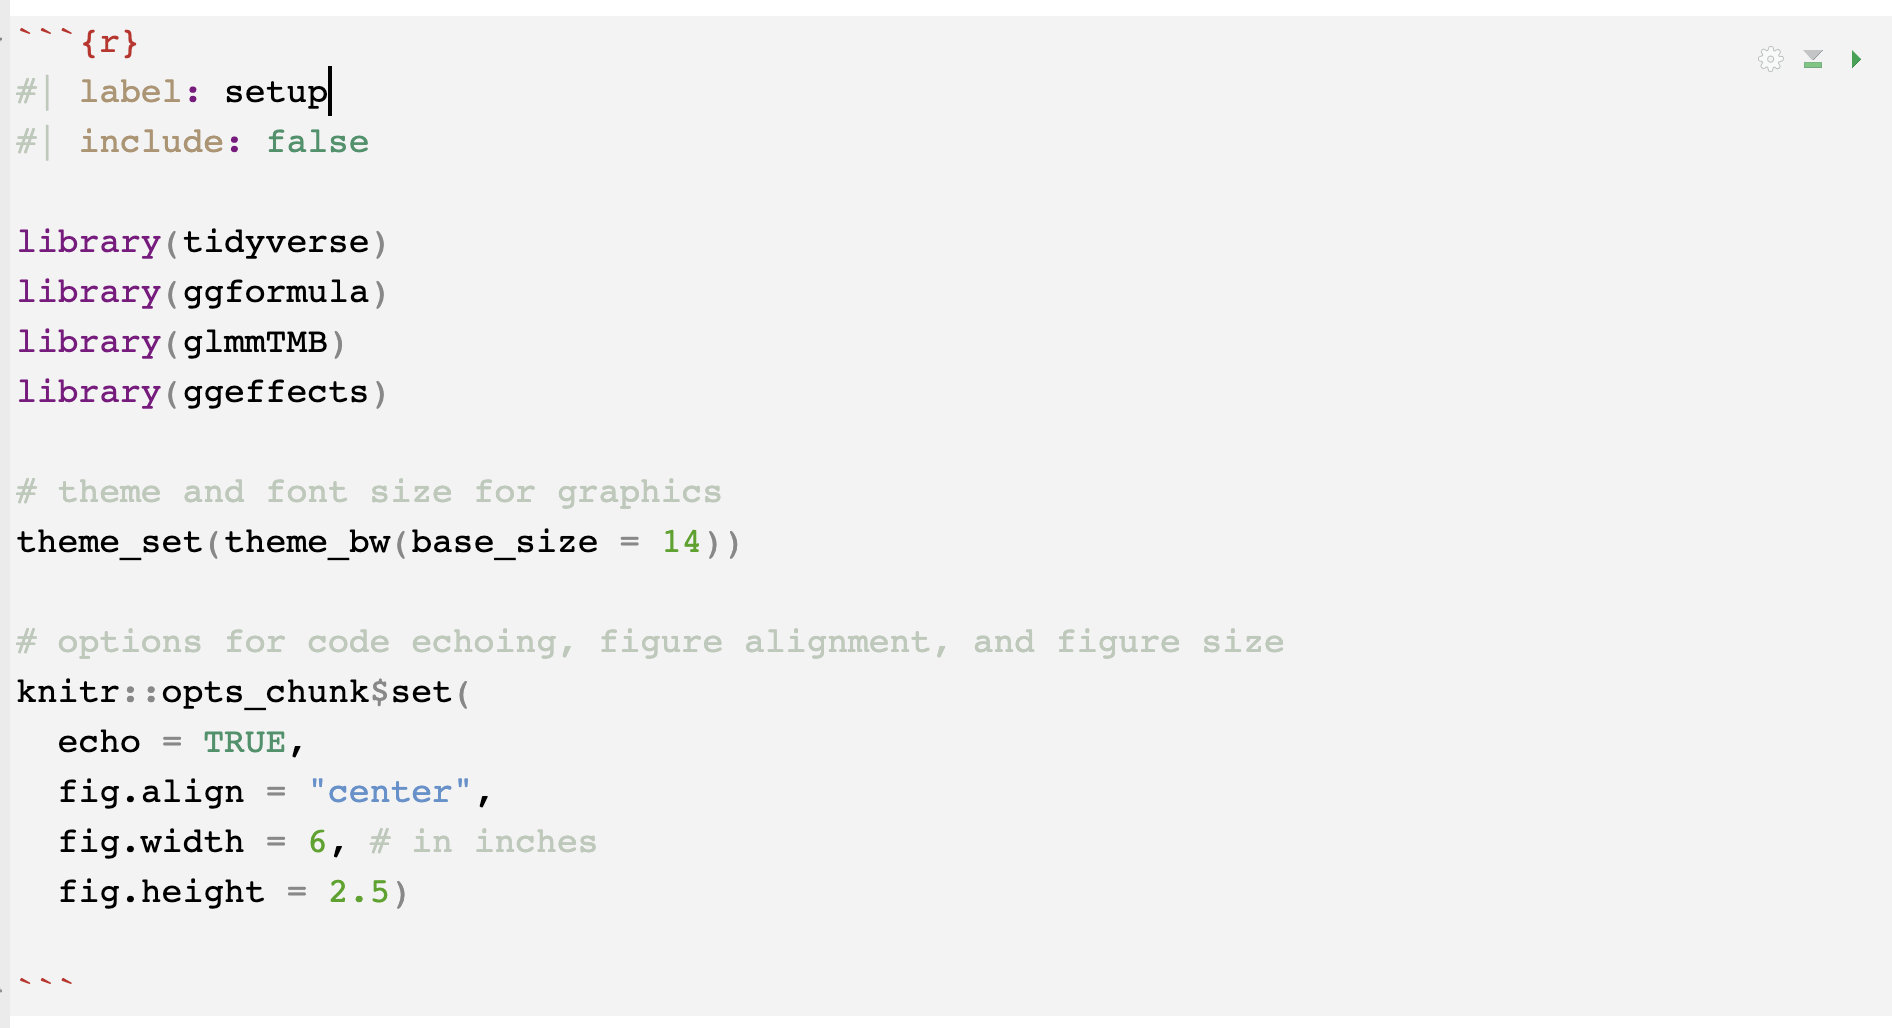
\includegraphics[width=0.8\linewidth,height=\textheight,keepaspectratio]{images/setup-chunk-2.png}

Next, Delete \textbf{everything} in the file \emph{other than} the YAML
header and your setup R code chunk.

Now the clutter is gone and you have space to include your own R code
and text.

(Before going further, make sure it still renders.)

\section{Run R Code}\label{run-r-code}

There are multiple ways to run and test R code from a markdown file.
Sometimes you want to render the whole file and get the PDF or HTML;
other times you want to run just a specific bit of code to make sure
it's working correctly.

\subsection{Running R Code from a qmd file: Render the
file}\label{running-r-code-from-a-qmd-file-render-the-file}

Every time you render the file, all R code will be run automatically.

A side note: PDF or HTML? Which is preferable?

I think PDFs are a little more portable and a good default option, and
their formatting is best for anything you are going to print out or
share via email (especially with less technically inclined folks).

However, later in the semester we may see how to create some pretty cool
interactive graphics and/or tables in R, and these can only be rendered
in HTML. For this class, you may use either one. (But not Word,
remember? Because you'll lose reproducibility\ldots)

\subsection{Running R Code from a qmd file: Run
Menu}\label{running-r-code-from-a-qmd-file-run-menu}

You can also use shortcuts/buttons to run specific chunk(s). Here is one
way to do it (option 1): Use the \emph{Run} pulldown menu at the top of
the file. (Choose the option you want based on what you are trying to
do).

\begin{center}
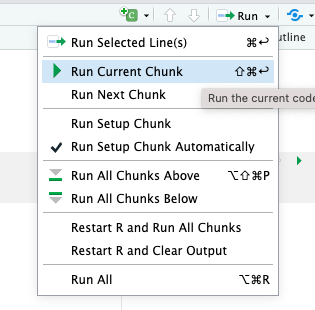
\includegraphics[width=0.85\linewidth,height=\textheight,keepaspectratio]{images/run-menu.png}
\end{center}

\subsection{Running Code from a qmd file: Shortcut
Button}\label{running-code-from-a-qmd-file-shortcut-button}

Here is another way to use shortcuts/buttons to run only a specific
chunk (option 2): Click on the green arrow at the upper right of a code
chunk to run the chunk.

\begin{center}
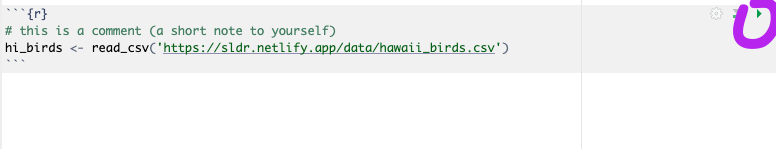
\includegraphics[width=0.85\linewidth,height=\textheight,keepaspectratio]{images/run-button-new.png}
\end{center}

\subsection{Running Code from a qmd file: Copy and
Paste}\label{running-code-from-a-qmd-file-copy-and-paste}

Finally, here's a third way to use shortcuts/buttons (option 3):

Copy the code you want to run, paste to the console window, and hit
Enter.

(Or, place your cursor in the line you want to run and hit ctrl + enter
(Windows) or cmd + enter (Mac).)

\section{Downloading files from
RStudio}\label{downloading-files-from-rstudio}

You will have to download your files if you want a copy on your own
computer, or to be able to upload a copy to Moodle to turn in.

To download, go to the \emph{File} tab, check the box for the file you
want, then select More - Export. from the menu at the top of the
\emph{File} tab.

\begin{center}
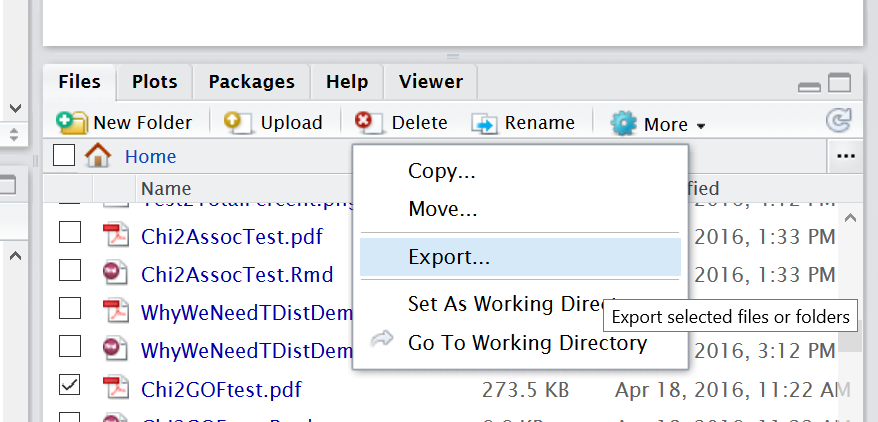
\includegraphics[width=0.85\linewidth,height=\textheight,keepaspectratio]{images/Export.png}
\end{center}

\section{Quarto Files Stand Alone!}\label{quarto-files-stand-alone}

We already covered this once, but we're covering it again because it's
one of the most common student mistakes in qmd files!

If you run R code in the console or the RStudio GUI (for example,
reading in a data set by pasting code into the console or using the
\emph{Import Dataset} button in the \emph{Environment} tab), \textbf{you
won't be able to use the results in your markdown file.}

Any and all commands you need, including reading in data, need to be
included in the file.

The reverse is also true. If you run just one R code chunk in a qmd file
using the ``run'' buttons mentioned above, or by copy-pasting into the
console, you are effectively running that code in the console.

If R gives an error saying it cannot find a certain funtion, variable,
or dataset, the most likely fix is to run the \emph{preceding} code
chunks (especially \texttt{setup}!) before the one you're stuck on.

\section{Data from a URL}\label{data-from-a-url}

You can load online datafiles in .csv format into R using the function
\texttt{read\_csv()}. The input to \texttt{read\_csv()} is the full url
where the file is located, in quotation marks. (Single or double quotes
-- it doesn't matter which you choose, as they are equivalent in R.)

For example, we will consider a dataset with counts of the numbers of
birds of different species seen at different locations in Hawai'i. It is
stored at \url{https://sldr.netlify.app/data/hawaii_birds.csv}, and can
be read into R using the command below.

\begin{Shaded}
\begin{Highlighting}[]
\NormalTok{hi\_birds }\OtherTok{\textless{}{-}} \FunctionTok{read\_csv}\NormalTok{(}\StringTok{\textquotesingle{}https://sldr.netlify.app/data/hawaii\_birds.csv\textquotesingle{}}\NormalTok{)}
\end{Highlighting}
\end{Shaded}

\subsection{When you read in data, store it to a named
object}\label{when-you-read-in-data-store-it-to-a-named-object}

Note that we didn't just run the \texttt{read\_csv()} function -- we
assigned the results a \textbf{name} so that instead of printing the
data table to the screen, R stores the dataset for later use.

\begin{Shaded}
\begin{Highlighting}[]
\NormalTok{hi\_birds }\OtherTok{\textless{}{-}} \FunctionTok{read\_csv}\NormalTok{(}\StringTok{\textquotesingle{}https://sldr.netlify.app/data/hawaii\_birds.csv\textquotesingle{}}\NormalTok{)}
\end{Highlighting}
\end{Shaded}

Here, we assigned the name \textbf{hi\_birds} to the dataset using an
``assignment arrow'' \texttt{\textless{}-} (the ``arrow'' points from
the object toward the name).

\section{Data from Google Sheets}\label{data-from-google-sheets}

There's also a simple way to read in data from a Google Sheet.

First, go to the Google Sheet online to prepare it by ``publishing it
online''.

In the \textbf{File} menu, choose ``Publish to the Web'':

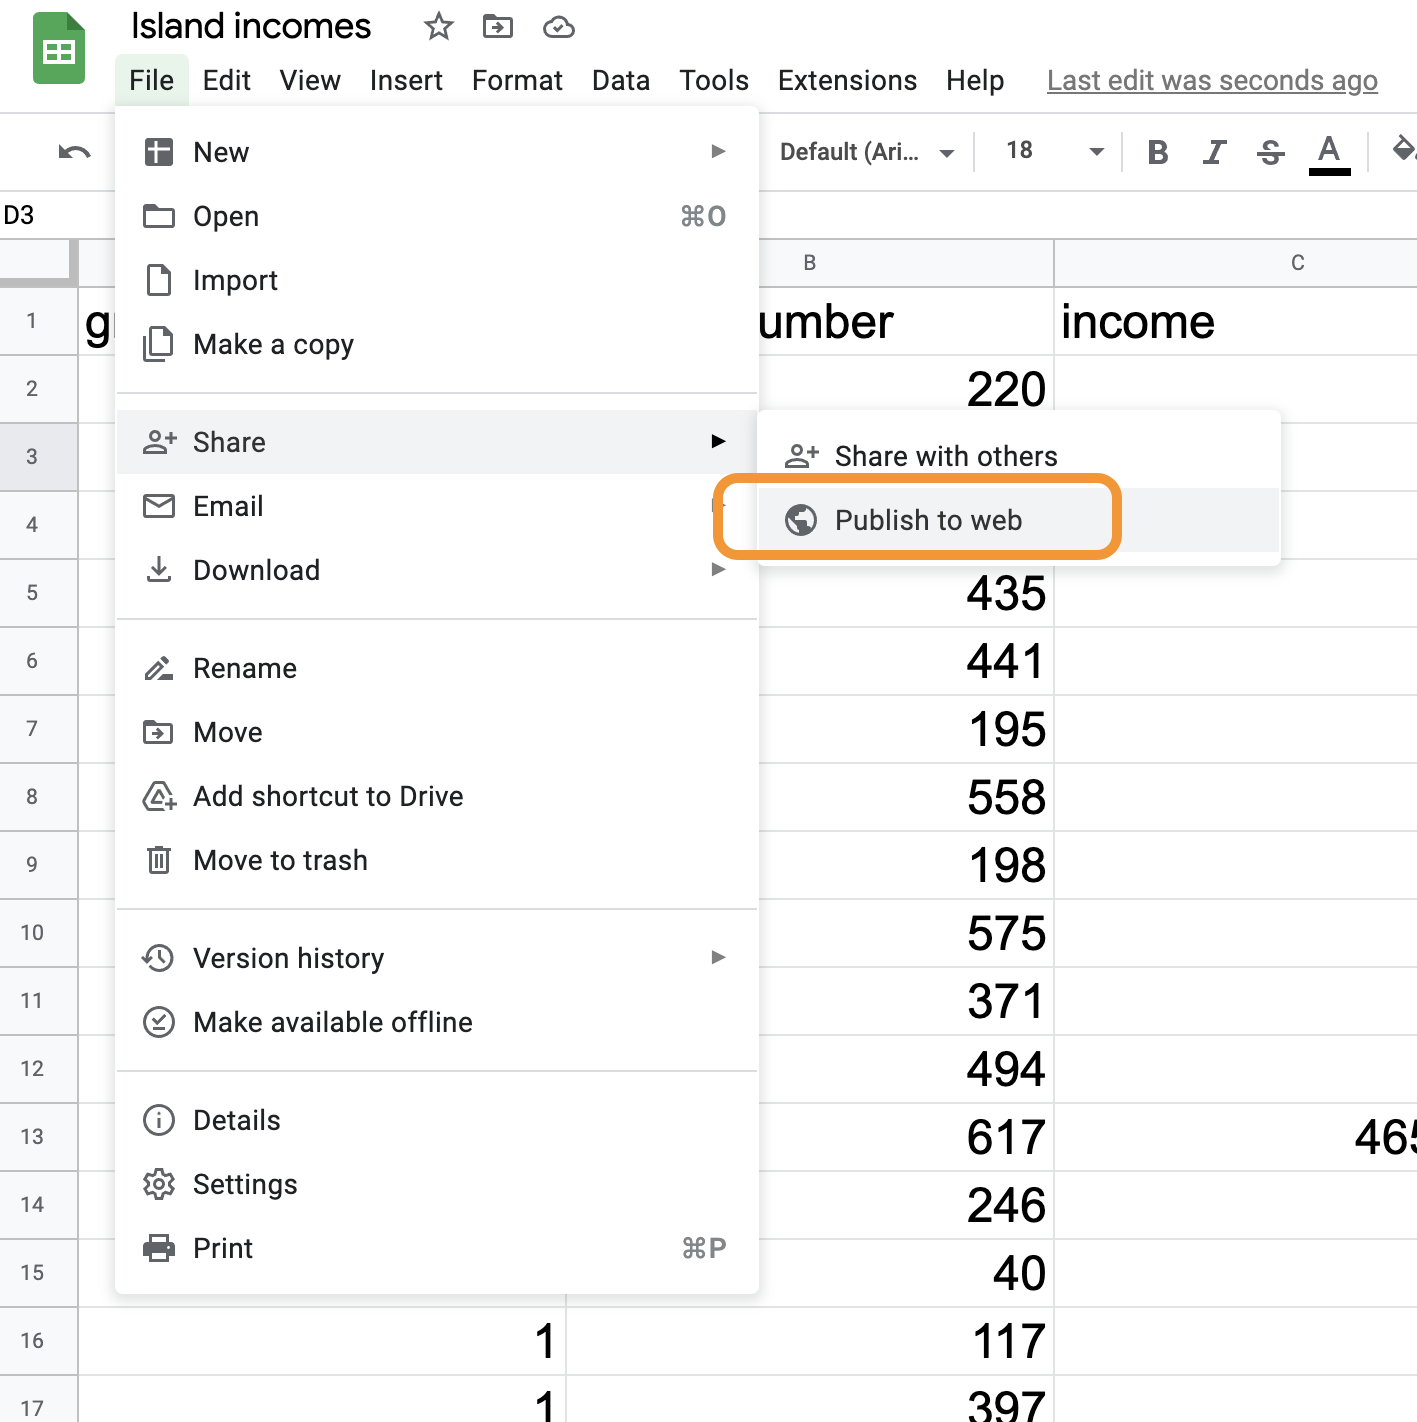
\includegraphics[width=5.20833in,height=\textheight,keepaspectratio]{images/publish-to-web.png}

In the pop-up window, choose to publish your ``Entire Document'' as a
.csv file:

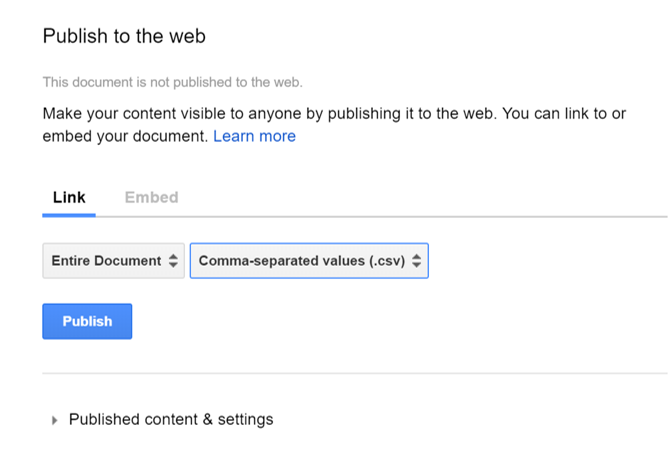
\includegraphics[width=5.20833in,height=\textheight,keepaspectratio]{images/publish-as-csv.png}

Finally, copy the resulting link.

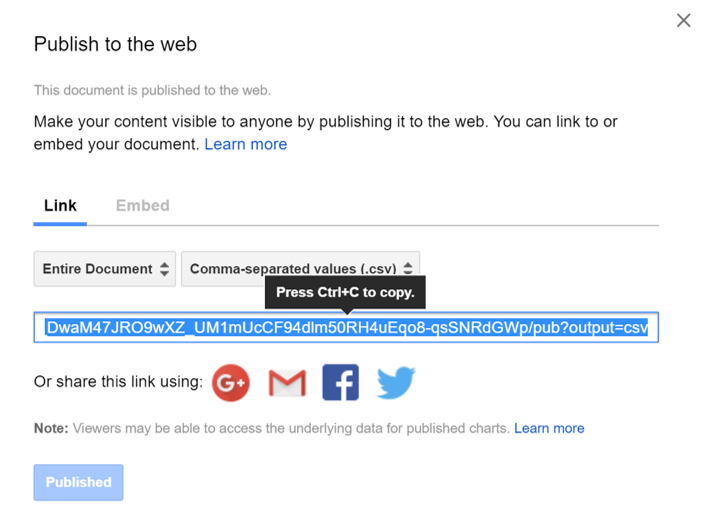
\includegraphics[width=5.20833in,height=\textheight,keepaspectratio]{images/get-link.png}

You can use \texttt{read\_csv()} with this link as input to read your
data into R.

\section{Data from a File}\label{data-from-a-file}

You can also upload your own data file to posit.cloud, or save it to
your computer if you installed R/RStudio, and then read it in to R using
\texttt{read\_csv()}. The basic process is:

\begin{itemize}
\tightlist
\item
  Use spreadsheet software to create the data table
\item
  Save the file as a csv file
\item
  Upload the csv file if working on posit.cloud
\item
  Use the \texttt{read\_csv()} function to read the file into R
\end{itemize}

\section{R functions}\label{r-functions}

After reading the data in, you can use R functions to have a look at it,
for example:

\begin{Shaded}
\begin{Highlighting}[]
\FunctionTok{head}\NormalTok{(hi\_birds)}
\FunctionTok{glimpse}\NormalTok{(hi\_birds)}
\FunctionTok{nrow}\NormalTok{(hi\_birds)}
\end{Highlighting}
\end{Shaded}

Try each of the lines of code above in R. What do the functions
\texttt{head()}, \texttt{glimpse()}, and \texttt{nrow()} \textbf{do}?
Try to figure it out based on the output they produce.

If you get stuck, consult R's built-in help files. Remember, you can
access the help for a function by running the code
\texttt{?functionName} -- for example, if you want help on
\texttt{head()}, run:

\begin{Shaded}
\begin{Highlighting}[]
\NormalTok{?head}
\end{Highlighting}
\end{Shaded}

\chapter{R Results in Quarto Text}\label{r-results-in-quarto-text}

\begin{Shaded}
\begin{Highlighting}[]
\FunctionTok{library}\NormalTok{(mosaic) }\CommentTok{\# for computing summary stats w/formula interface}
\end{Highlighting}
\end{Shaded}

\section{Including results of R calculations in your
text}\label{including-results-of-r-calculations-in-your-text}

You may want to include the results of R calculations in the TEXT part
of a report. Then, if the calculated value changes, the text can be
automatically updated to match.

Let's say you compute the mean of some kids' foot lengths:

\begin{Shaded}
\begin{Highlighting}[]
\FunctionTok{mean}\NormalTok{(}\SpecialCharTok{\textasciitilde{}}\NormalTok{length, }\AttributeTok{data =}\NormalTok{ KidsFeet)}
\end{Highlighting}
\end{Shaded}

\begin{verbatim}
[1] 24.72308
\end{verbatim}

\subsection{Simple but Inefficient}\label{simple-but-inefficient}

You may want to cite the result in the text part of your file\ldots so
you would type:

The mean length of the kids' feet was ` r mean(\textasciitilde length,
data=KidsFeet) ` cm.

To get:

The mean length of the kids' feet was 24.7230769 cm.

\subsection{Side Note: back-ticks}\label{side-note-back-ticks}

\emph{Those accent marks (before the ``r'' and at the end of the R-code
stuff) are not normal single quotes or apostrophes; they are
``back-ticks'' or ``graves'' ( ` ), just like those used to help define
the start and end of R code chunks in your Quarto file. There should not
actually be a space between the ` and the r.}

\subsection{More Efficient}\label{more-efficient}

It's annoying (and sometimes not really practical) to (re)type the
entire R command in the text part of your file. An option is to save the
quantity you want to refer to as a variable in R:

\begin{Shaded}
\begin{Highlighting}[]
\NormalTok{mean\_length }\OtherTok{\textless{}{-}} \FunctionTok{mean}\NormalTok{(}\SpecialCharTok{\textasciitilde{}}\NormalTok{length, }\AttributeTok{data =}\NormalTok{ KidsFeet)}
\end{Highlighting}
\end{Shaded}

Then you can write: The mean foot length of the kids was ` r
mean\_length` cm.

To get: The mean foot length of the kids was 24.7230769 cm.

\section{Rounding}\label{rounding}

What if you want to report numeric values with a more reasonable number
of decimal places? Use \texttt{round()}: The mean foot length of the
kids was ` r round(mean\_length, digits = 2)` cm

and you get: The mean foot length of the kids was 24.72 cm

You can also consider using the function \texttt{signif()} if you want
to specify the number of significant digits rather than the number of
decimal places.

\section{R results with more than one value
inside}\label{r-results-with-more-than-one-value-inside}

What if you want to cite a value from an object that contains more than
one value?

\subsection{Vectors}\label{vectors}

For example, what if you computed means for both boys and girls? The
output would be a vector of two means, then.

You can use hard brackets ( {[} \ldots{} {]} ) to refer to the first,
second, etc. entries. For example:

\begin{Shaded}
\begin{Highlighting}[]
\NormalTok{girlboy.means }\OtherTok{\textless{}{-}} \FunctionTok{mean}\NormalTok{(}\SpecialCharTok{\textasciitilde{}}\NormalTok{ length }\SpecialCharTok{|}\NormalTok{ sex,}
                      \AttributeTok{data =}\NormalTok{ KidsFeet)}
\end{Highlighting}
\end{Shaded}

You type: The girls' mean foot length was ` r girlboy.means{[}``G''{]}
`, and the boys' was ` r girlboy.means{[}``B''{]} `

to get: The girls' mean foot length was 24.3210526, and the boys' was
25.105.

\emph{You can also use numeric indices -- for example, ` r
girlboy.means{[}2{]} ` instead of ` r girlboy.means{[}``G''{]} ` to get
the girls' value -- but using names when you can is often safer because
you don't have to worry about whether things are stored in the order you
think that they are!}

\subsection{Matrices, Tables, data.frames,
tibbles\ldots{}}\label{matrices-tables-data.frames-tibbles}

If you are referring to a data table or other object with multiple rows
and columns, you can use the syntax
\texttt{{[}row.numbers,\ column.numbers{]}} to extract a row, a column,
or a specific value of interest. If you leave either
\texttt{row.numbers} or \texttt{column.numbers} blank, all rows/columns
will be included.

For example, consider a table showing some data from a survey of intro
stat students (\texttt{Ticket} tells whether they have gotten a speeding
ticket while driving a car, and \texttt{Texted} tells whether they have
texted while driving a car):

\begin{Shaded}
\begin{Highlighting}[]
\NormalTok{student\_survey }\OtherTok{\textless{}{-}} \FunctionTok{read.csv}\NormalTok{(}\StringTok{\textquotesingle{}https://sldr.netlify.app/data/IntroStatStudents.csv\textquotesingle{}}\NormalTok{, }
              \AttributeTok{na.strings =} \FunctionTok{list}\NormalTok{(}\StringTok{\textquotesingle{}\textquotesingle{}}\NormalTok{, }\StringTok{\textquotesingle{}NA\textquotesingle{}}\NormalTok{))}
\FunctionTok{tally}\NormalTok{(}\SpecialCharTok{\textasciitilde{}}\NormalTok{Ticket }\SpecialCharTok{|}\NormalTok{ Texted, }
      \AttributeTok{data =}\NormalTok{ student\_survey, }
      \AttributeTok{format =} \StringTok{\textquotesingle{}proportion\textquotesingle{}}\NormalTok{)}
\end{Highlighting}
\end{Shaded}

\begin{verbatim}
               Texted
Ticket                  No        Yes
  I don't drive 0.03703704 0.00000000
  No            0.77777778 0.71900826
  Yes           0.14814815 0.28099174
  <NA>          0.03703704 0.00000000
\end{verbatim}

What if we want to print just the first column of data?

(\emph{Note: Don't count the row and column names when numbering the
rows and columns}.)

\begin{Shaded}
\begin{Highlighting}[]
\FunctionTok{tally}\NormalTok{(}\SpecialCharTok{\textasciitilde{}}\NormalTok{Ticket }\SpecialCharTok{|}\NormalTok{ Texted, }
      \AttributeTok{data =}\NormalTok{ student\_survey,}
      \AttributeTok{format =} \StringTok{\textquotesingle{}proportion\textquotesingle{}}\NormalTok{)[,}\DecValTok{1}\NormalTok{]}
\end{Highlighting}
\end{Shaded}

\begin{verbatim}
I don't drive            No           Yes          <NA> 
   0.03703704    0.77777778    0.14814815    0.03703704 
\end{verbatim}

Or better (and clearer\ldots)

\begin{Shaded}
\begin{Highlighting}[]
\FunctionTok{tally}\NormalTok{(}\SpecialCharTok{\textasciitilde{}}\NormalTok{Ticket }\SpecialCharTok{|}\NormalTok{ Texted, }
      \AttributeTok{data =}\NormalTok{ student\_survey,}
      \AttributeTok{format =} \StringTok{\textquotesingle{}proportion\textquotesingle{}}\NormalTok{)[, }\StringTok{"No"}\NormalTok{]}
\end{Highlighting}
\end{Shaded}

\begin{verbatim}
I don't drive            No           Yes          <NA> 
   0.03703704    0.77777778    0.14814815    0.03703704 
\end{verbatim}

What about the third row (for people who have gotten a ticket)?

\begin{Shaded}
\begin{Highlighting}[]
\FunctionTok{tally}\NormalTok{(}\SpecialCharTok{\textasciitilde{}}\NormalTok{Ticket }\SpecialCharTok{|}\NormalTok{ Texted, }
      \AttributeTok{data =}\NormalTok{ student\_survey, }
      \AttributeTok{format =} \StringTok{\textquotesingle{}proportion\textquotesingle{}}\NormalTok{)[}\StringTok{"Yes"}\NormalTok{,]}
\end{Highlighting}
\end{Shaded}

\begin{verbatim}
       No       Yes 
0.1481481 0.2809917 
\end{verbatim}

What about the proportion of students with tickets, among those who've
texted while driving? (Row 3, Column 2 = row ``Yes'' and column
``Yes'')? Let's first save the table so we don't have to
recompute\ldots{}

\begin{Shaded}
\begin{Highlighting}[]
\NormalTok{driver\_table }\OtherTok{\textless{}{-}} \FunctionTok{tally}\NormalTok{(}\SpecialCharTok{\textasciitilde{}}\NormalTok{Ticket }\SpecialCharTok{|}\NormalTok{ Texted, }
      \AttributeTok{data =}\NormalTok{ student\_survey, }
      \AttributeTok{format =} \StringTok{\textquotesingle{}proportion\textquotesingle{}}\NormalTok{)}
\end{Highlighting}
\end{Shaded}

Type: The proportion of students who have texted while driving who have
gotten a speeding ticket is ` r driver\_table{[}``Yes'',``Yes''{]} `.

To get: The proportion of students who have texted while driving who
have gotten a speeding ticket is 0.2809917.

(\emph{Like before, if it's possible to use names instead of numeric
indices, try to do so!})

\chapter{Math Notation in Quarto}\label{math-notation-in-quarto}

\section{Greek Letters, common symbols, subscripts and
superscripts}\label{greek-letters-common-symbols-subscripts-and-superscripts}

You might be wondering\ldots{}

\begin{quote}
\begin{quote}
How can I include Greek letters and other symbols in the text part of my
Quarto (or RMarkdown) document?
\end{quote}
\end{quote}

Basically, you enclose the name of the symbol you want with \$...\$

(if you use LaTeX, this will be very familiar):

\begin{longtable}[]{@{}ll@{}}
\toprule\noalign{}
Type this in qmd: & To get this when rendered: \\
\midrule\noalign{}
\endhead
\bottomrule\noalign{}
\endlastfoot
\$\textbackslash hat\{p\}\$ & \(\hat{p}\) \\
\$\textbackslash bar\{x\}\$ & \(\bar{x}\) \\
\$\textbackslash alpha\$ & \(\alpha\) \\
\$\textbackslash beta\$ & \(\beta\) \\
\$\textbackslash gamma\$ & \(\gamma\) \\
\$\textbackslash Gamma\$ & \(\Gamma\) \\
\$\textbackslash mu\$ & \(\mu\) \\
\$\textbackslash sigma\$ & \(\sigma\) \\
\$\textbackslash sigma\^{}2\$ & \(\sigma^2\) \\
\$\textbackslash rho\$ & \(\rho\) \\
\$\textbackslash epsilon\$ & \(\epsilon\) \\
\$\textbackslash sim\$ & \(\sim\) \\
\$\textbackslash mu\_D\$ & \(\mu_D\) \\
\$\textbackslash mu\_\{longsubscript\}\$ & \(\mu_{longsubscript}\) \\
\$\textbackslash hat\{p\}\_\{longsubscript\}\$ &
\(\hat{p}_{longsubscript}\) \\
\$\textbackslash mu\textbackslash neq 0\$ & \(\mu \neq 0\) \\
\$\textbackslash mu\textbackslash geq 5\$ & \(\mu \geq 5\) \\
\$\textbackslash mu\textbackslash leq 1\$ & \(\mu \leq 1\) \\
\$\textbackslash cup\$ & \(\cup\) \\
\$\textbackslash cap\$ & \(\cap\) \\
\$\textbackslash vert\$ & \(\vert\) \\
\$\textbackslash sim\$ & \(\sim\) \\
\$\textbackslash frac\{numerator\}\{denominator\}\$ &
\(\frac{numerator}{denominator}\) \\
\end{longtable}

For other Greek letters, just spell out the name of the letter that you
want (following the models above). If you want a capital Greek letter,
capitalize the first letter of its name when you write it out
(e.g.~Sigma instead of sigma).

\emph{Note: Avoid spaces before the final \$ or after the initial \$.}

\section{Summations and Products}\label{summations-and-products}

\begin{longtable}[]{@{}ll@{}}
\toprule\noalign{}
Type This: & To get this in your PDF: \\
\midrule\noalign{}
\endhead
\bottomrule\noalign{}
\endlastfoot
\$\textbackslash sum\_\{i=1\}\^{}\{n\} x\_i\$ &
\(\sum_{i=1}^{n} x_i\) \\
\$\textbackslash prod\_\{i=1\}\^{}\{n\} f(i)\}\$ &
\(\prod_{i=1}^{n} f(i)\) \\
\end{longtable}

These will format as seen above if used in inline math mode (enclosed in
single \$s). If you put them in display math mode by using two \$\$ at
the start and end instead of just one, then the result will be displayed
centered on its own line and the limits of the summation/product will be
above/below the \(\Sigma\) or \(\Pi\):

\[\prod_{i=1}^{n} f(i)\]

\section{Long equations}\label{long-equations}

You can use double \$ to bracket equations you want to display on a line
of their own. Inside can be multiple mathematical expressions. For
example:

\begin{Shaded}
\begin{Highlighting}[]
\NormalTok{$$\textbackslash{}hat\{y\} = \textbackslash{}beta\_0 + \textbackslash{}beta\_1x\_1\textbackslash{},$$}

\NormalTok{$$\textbackslash{}hat\{epsilon\} = \textbackslash{}hat\{y\}\_\{i\} {-} y\_i$$}

\NormalTok{$$\textbackslash{}epsilon \textbackslash{}sim N(0, \textbackslash{}sigma)$$}
\end{Highlighting}
\end{Shaded}

gives

\[\hat{y} = \beta_0 + \beta_1x_1\]

\[\hat{\epsilon}_{i} = \hat{y}_{i} - y_i\]

\[\epsilon \sim N(0, \sigma)\]

\emph{Note: Avoid spaces before the final \$ or after the initial \$.
Also note, the equation will NOT be inside a code chunk\ldots I only did
that here because it's hard to get the} \textbf{un-rendered source
version} \emph{to appear neatly in the text part of a rendered Quarto
file otherwise.}

\part{Designing Effective Visualizations}

\section*{Section Learning Outcomes}\label{section-learning-outcomes}
\addcontentsline{toc}{section}{Section Learning Outcomes}

\markright{Section Learning Outcomes}

After this section, you will be able to:

\begin{enumerate}
\def\labelenumi{\arabic{enumi}.}
\tightlist
\item
  Critique statistical graphics based on design principles.
\item
  Recognize common misleading design choices for data visualizations
\item
  Recognize data visualization that tells a true story, identifying
  elements that emphasize the main finding and make the figure easy to
  interpret at a glance
\end{enumerate}

\section*{Reference Materials}\label{reference-materials-1}
\addcontentsline{toc}{section}{Reference Materials}

\markright{Reference Materials}

\begin{itemize}
\tightlist
\item
  \href{https://bookdown.org/roback/bookdown-BeyondMLR/ch-MLRreview.html\#explorech1}{\emph{Beyond
  Multiple Linear Regression} Ch. 1.5}
\item
  \emph{Ecological Models \& Data in R} Ch. 2 discusses graphics, but is
  not recommended as the approach to reading in data, writing R code,
  and generating graphs in R is very different to that used in this
  course.
\item
  A comprehensive, and free, supplemental reference is
  \href{https://clauswilke.com/dataviz/}{Fundamentals of Data
  Visualization by Claus Wilke}
\end{itemize}

It's suggested that you refer to the above materials as needed
\emph{after} doing this section, with particular focus on the topics you
found most challenging.

\section*{Inspiration}\label{inspiration}
\addcontentsline{toc}{section}{Inspiration}

\markright{Inspiration}

\begin{quote}
Above all, show the data.

E. Tufte, \href{https://www.edwardtufte.com/tufte/books_vdqi}{\emph{The
Visual Display of Quantitative Information}}
\end{quote}

But\ldots{}

\begin{quote}
The Numbers Don't Speak for Themselves.

C. D'Ignazio and L. Klein,
\href{https://data-feminism.mitpress.mit.edu/pub/czq9dfs5/release/2}{\emph{Data
Feminism}}
\end{quote}

In visualizing data, we use graphics to gain and communicate an honest
understanding of data in context.

\section*{Motivation: Imagine First!}\label{motivation-imagine-first}
\addcontentsline{toc}{section}{Motivation: Imagine First!}

\markright{Motivation: Imagine First!}

Figures are a crucial tool for exploring your data \emph{and}
communicating what you learn from the data.

Whether you are doing a quick check to assess basic features of a
dataset or creating a key figure for an important presentation, the best
practice is to work thoughtfully.

\subsection*{\texorpdfstring{The \textbf{I.C.E.E.
method}:}{The I.C.E.E. method:}}\label{the-i.c.e.e.-method}
\addcontentsline{toc}{subsection}{The \textbf{I.C.E.E. method}:}

\begin{itemize}
\tightlist
\item
  \textbf{I}\emph{magine} how you want your graph to look, \emph{before}
  you
\item
  \textbf{C}\emph{ode}. Once you have the basic starting point,
\item
  \textbf{E}\emph{valuate} your work, and
\item
  \textbf{E}\emph{laborate} (refine it).
\end{itemize}

Repeat until the figure is as awesome as it needs to be.

\subsection*{NO To Mindless Copy/Paste}\label{no-to-mindless-copypaste}
\addcontentsline{toc}{subsection}{NO To Mindless Copy/Paste}

Too many of us fall into the trap of starting to write code (or
copy/pasting it!) \emph{before} pausing to think carefully about the
desired outcome, then settling for the first vaguely relevant result (or
\href{https://twitter.com/accidental__art?lang=en}{delighting in the
unintended outcome}\ldots).

\begin{quote}
\begin{quote}
You can do better than mindless copying! Only \emph{mindful}
copy-pasting allowed.
\end{quote}
\end{quote}

This section provides some advice to get you started. It can also
provide inspiration for constructive critique of others' graphics.

Here we focus only on the \textbf{I\_EE} parts of the process, where you
design and assess graphics. Code will come later.

\section*{Appearance Goals}\label{appearance-goals}
\addcontentsline{toc}{section}{Appearance Goals}

\markright{Appearance Goals}

Specifically, how \emph{exactly} should a graphic look? There are so
many choices: color, size, text and more. What are best practices for
creating something beautiful, that represents the data honestly, and is
easy to understand?

This section will provide some rules of thumb to help you
\textbf{Evaluate} statistical graphics. It will also teach you to spot
common problems and suggest ways to fix them, allowing you to provide
\emph{constructive} critique (to yourself or to others!) about how to
\textbf{Elaborate} and refine data visualizations.

\subsection*{You still have your
freedom!}\label{you-still-have-your-freedom}
\addcontentsline{toc}{subsection}{You still have your freedom!}

As you digest all these rules and tips, you may wonder: ``Do I
\emph{have} to always obey every one?'' Well\ldots No, of course not. Be
creative!

Sometimes it's OK to break these rules \emph{when you have thought it
through} and \emph{with a good justification}.

A good justification means that in your particular case, breaking a
certain rule will make your graph more informative, easier to
understand, or better at telling the story you're highlighting.

\section*{Learning Objectives}\label{learning-objectives}
\addcontentsline{toc}{section}{Learning Objectives}

\markright{Learning Objectives}

This section will give you some basic tools to:

\begin{enumerate}
\def\labelenumi{\arabic{enumi}.}
\tightlist
\item
  \textbf{Graph data with integrity}, avoiding misleading design choices
\item
  \textbf{Tell the right story}, including elements that \emph{emphasize
  your main finding} and make your figure \emph{easy to interpret at a
  glance}
\end{enumerate}

\chapter{\texorpdfstring{What is
\emph{Necessary}?}{What is Necessary?}}\label{what-is-necessary}

\section{Bye, Junk!}\label{bye-junk}

Our first principle is: if it doesn't \emph{need} to be in your graph,
it shouldn't be there. Keep things as simple as possible. What are some
justifications for a \emph{need} to include an element in a plot?

\begin{itemize}
\tightlist
\item
  It is crucial to the story you are telling, or the research question
  you are answering.
\item
  It emphasizes your main point. For example, some plots may not need
  color, and in others it may add crucial visual contrast to highlight a
  main point.
\item
  It makes the graph easier to read and understand
\item
  It makes the main message of the graph more memorable
\end{itemize}

\textbf{If you need it, include it, but if not, keep it simple!}

Imagine you are using \emph{very} expensive ink to print every element
of the graph. Is every drop of in you're using really worth it? If not,
take it out. As influential data visualization thinker Edward Tufte put
it in \href{https://www.edwardtufte.com/tufte/books_vdqi}{\emph{The
Visual Display of Quantitative Information}},

\begin{quote}
A large share of ink on a graphic should present data-information, the
ink changing as the data change. Data-ink is the non-erasable core of a
graphic\ldots{}
\end{quote}

In other words, don't let annotations, labels, grids, etc. overwhelm the
visual impact of your data -- Don't do this:

\includegraphics[width=4.16667in,height=\textheight,keepaspectratio]{index_files/mediabag/Data-ink-1024x768.png}

\emph{Cartoon source: \url{https://freshspectrum.com/data-ink-ratio/}}

\subsection{Check: Critique the Pie}\label{check-critique-the-pie}

The figure below, from
\href{https://www.forbes.com/sites/tomiogeron/2012/02/02/does-ios-crash-more-than-android-a-data-dive/\#4997f14d5385}{a
\emph{Forbes} article on mobile operating system crashes}, \textbf{is
pretty awful}.

\pandocbounded{\includegraphics[keepaspectratio]{index_files/mediabag/crashes-ios-android-.png}}

\subsubsection{A Conclusion?}\label{a-conclusion}

What is \textbf{one main conclusion} from the graph above?

(It's pretty confusing to interpret, so you may have to study carefully
to find something\ldots)

\subsubsection{Remove\ldots What?}\label{removewhat}

Now that you have identified one main conclusion from the graph\ldots{}

What is one element of the plot that:

\begin{itemize}
\tightlist
\item
  obscures that conclusion,
\item
  is NOT necessary, and
\item
  could be removed to improve the plot?
\end{itemize}

Answer constructively - as if the person who made the plot was
incredibly smart and someone you admire, and to whom you wanted to be
kind but helpful.

\section{Grids and Boxes}\label{grids-and-boxes}

Should your graphics include boxes, axis lines, and grid lines?

Well, it depends\ldots{}

\begin{itemize}
\tightlist
\item
  Removing unnecessary axes, grids, and labels yields a cleaner plot
  that may be easier to take in at a glance -- there is less to distract
  from the main story
\item
  \textbf{But\ldots{}} omitting needed baselines, tick marks, gridlines,
  and labels can cause confusion and make it hard to identify categories
  or estimate numeric values
\item
  Scientific graphics usually need axis lines, with tick marks
\item
  If a viewer will need to refer to an axis to estimate heights of bars
  or locations of points, then consider using gridlines for that axis.
\item
  Instead of an entire grid, it may be more effective to include single
  lines indicating important threshold values
\item
  Consider using a color that nearly blends into the background for grid
  lines, so that they detract as little attention as possible from the
  data
\end{itemize}

\subsection{Example}\label{example}

\href{http://www.storytellingwithdata.com/blog/2011/07/gridlines-are-gratuitous}{Storytelling
with Data} provide an example of a cluttered figure where the trend over
time pops out more as unnecessary grids and boxes are made less visible,
then removed:

\includegraphics[width=3.125in,height=\textheight,keepaspectratio]{index_files/mediabag/image-asset.jpg}

Optionally, if you'd like more examples, read
\href{http://www.perceptualedge.com/articles/dmreview/grid_lines.pdf}{S.
Few's 3.5-page article on when grid lines are helpful.}

\chapter{Color}\label{color}

\section{Using Color}\label{using-color}

Color - used with care - can be an incredibly effective part of a data
visualization.

\begin{itemize}
\tightlist
\item
  Ensure your color choices \textbf{highlight the story} you want to
  tell

  \begin{itemize}
  \tightlist
  \item
    Consider using black and grey to help some elements fade into the
    background - for example, grid lines and labels that must be present
    but aren't the most important elements.
  \item
    Or, color all groups but the one you want to highlight in grey, and
    use a bold color for the ``main'' group\ldots{}
  \end{itemize}
\item
  Choose color combinations that look good and are
  \textbf{distinguishable by color-blind viewers and in greyscale}

  \begin{itemize}
  \tightlist
  \item
    Defaulting to pre-defined color palettes provided by your software
    may be better than haphazardly choosing colors manually
  \item
    Consider being redundant - use size and/or shape as well as color to
    indicate groups so figures are legible in greyscale, too.
  \end{itemize}
\item
  Use color \textbf{consistently}.
\item
  Example: if ``young'' cases are red in one graph, don't use red for
  ``old'' in the next graph. And if many graphs are colored by the same
  grouping variable, use the same colors in all of them.
\end{itemize}

The video below, created by
\href{https://www.youtube.com/c/storytellingwithdata}{Storytelling with
Data}, gives explanations and examples.

\begin{itemize}
\tightlist
\item
  If you have time, watch from 11:48 to 28:41 (about 17 minutes). This
  segment will play automatically in the clip below.
\item
  If you're in a rush, the most important sections (about 10 minutes)
  are:

  \begin{itemize}
  \tightlist
  \item
    13:57 - 15:12 (Sparing use of color)
  \item
    18:44 - 21:25; see also the
    \href{https://www.informationisbeautiful.net/visualizations/colours-in-cultures/}{infographic
    of color in culture}
  \item
    22:25 - 23:10 (Color blindness - to view your graphs as someone with
    color blindness would, take a screen shot and try the
    \href{https://www.color-blindness.com/coblis-color-blindness-simulator/}{simulator
    online}
  \item
    23:50 - 28:41 (Consistency)
  \end{itemize}
\end{itemize}

\textbf{Which of the following are lessons from the Storytelling with
Data video on Being Clever with Color? Mark all correct answers
``TRUE''.}

Color grabs attention. TRUE / FALSE

Color signals where to look. TRUE / FALSE

Color should be used sparingly. TRUE / FALSE

Too much color, and everything is highlighted - the viewer does not know
what to pay attention to. TRUE / FALSE

Color can show quantitative values, too, not just categories. TRUE /
FALSE

Colors have tone and meaning. TRUE / FALSE

Not everyone can see colors. TRUE / FALSE

Use color consistently. TRUE / FALSE

Simple black and white is always the best choice. TRUE / FALSE

Click for explanations of solutions above.

\begin{itemize}
\tightlist
\item
  The human eye is naturally drawn to colors.
\item
  Since color grabs attention, we expect it to direct us toward the most
  important stuff that is worthy of our attention.
\item
  But\ldots Too much color, and everything is highlighted - the viewer
  does not know what to pay attention to.
\item
  Also, remember that the meaning and interpretation of colors varies by
  culture.
\item
  Since some people can not see color, use color-blind friendly palettes
  and redundant coding (shape, text) where possible without cluttering
  the figure.
\item
  Inconsistent use of color can be confusing and distracting.
\item
  Sometimes black and white is great - but often color helps you tell a
  story!
\end{itemize}

\chapter{Text Elements}\label{text-elements}

\section{Titles, Labels, Size}\label{titles-labels-size}

When using text in a figure, ensure it is easy to read. Make sure no
unneccessary text is included.

\begin{itemize}
\tightlist
\item
  Default size of text in figures produced by statistical software
  \emph{is almost always too small}. Make sure your text is \emph{big
  enough to be easily legible in the context where you will present it}
  (on the page in a report, on a slide for a presentation, etc.)
\item
  Other than the title of the vertical (y) axis, all the text in a plot
  should be horizontal. This makes it easier to read.
\item
  Axis labels should be self-explanatory

  \begin{itemize}
  \tightlist
  \item
    Viewers should be able to guess what they mean accurately without
    looking at anything but the figure
  \item
    Use words instead of numeric codes or cryptic abbreviations
  \end{itemize}
\item
  Axis labels should also be as short as possible while remaining easy
  to understand
\item
  Every plot should have a title. Sometimes this might be a literal
  title at the top of the graph, but those are relatively rare. More
  often in scientific work, a text caption appears below the figure. The
  first phrase/sentence of the caption acts as the figure's title
\end{itemize}

Remember the melanoma rates over time figure we saw earlier?

\includegraphics[width=3.125in,height=\textheight,keepaspectratio]{index_files/mediabag/image-asset.jpg}

\textbf{What helpful changes did Storytelling with Data make to the text
labels as they improved the figure?}

The x axis labels are rotated so they are horizonal. TRUE / FALSE

The title color is changed to blue and the axis labels to grey. TRUE /
FALSE

The box around the plot is removed. TRUE / FALSE

Click for explanations of solutions above.

\begin{itemize}
\tightlist
\item
  Rotating axis labels so they are horizontal is generally an
  improvement. To make this happen, the number of tick marks and labels
  on the x axis was also reduced. Notice the labels are much easier to
  read.
\item
  The color changes helped too. The blue links the title with the trend
  it describes, and the grey makes the axis titles less prominent and
  lets the viewer focus on the data. Continue to the next section for
  more on using color\ldots{}
\item
  The box is gone, and it is a big improvement to the plot! But
  technically, you were asked about changes to the text labels\ldots{}
\end{itemize}

\section{When Things Overlap}\label{when-things-overlap}

Especially when graphing variables with long category values, you may
end up with ugly, illegible overlapping labels.

Some solutions, in rough order of preference, are to:

\begin{itemize}
\tightlist
\item
  adjust the figure width or height so everything fits
\item
  switch x and y coordinates so the ``long'' labels are on the y axis
  (in R, this resizes the plot area so that labels fit); or,
\item
  rotate the too-long labels, which eliminates the overlap \emph{but
  makes them harder to read than horizontal text.}
\item
  make the font smaller (\emph{but this might make it annoyingly hard to
  read, or make your viz feel cluttered!})
\end{itemize}

\section{When Text Runs ``off the
edge''}\label{when-text-runs-off-the-edge}

Sometimes a title or axis label is too long and runs off the edge of the
figure. Using a smaller font is \emph{not} often an ideal solution. If
you can't just use a shorter label, consider adding line breaks.

\section{Examples}\label{examples}

\begin{center}
\pandocbounded{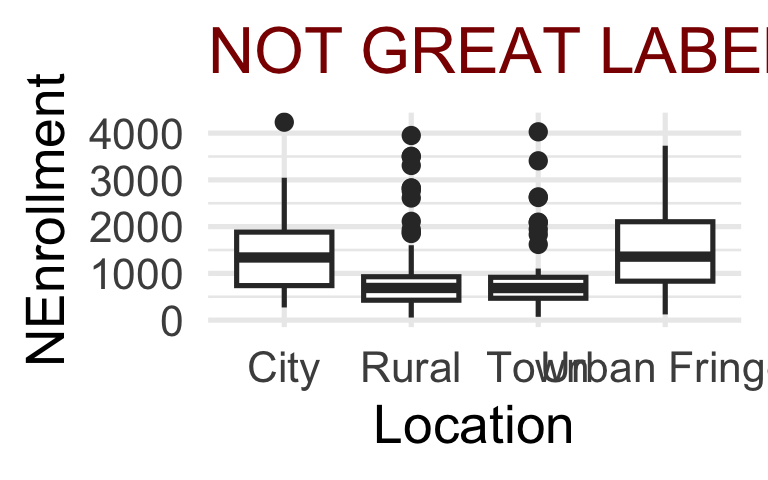
\includegraphics[keepaspectratio]{graph-design-text-elements_files/figure-pdf/bad-labels-1.pdf}}
\end{center}

\begin{center}
\pandocbounded{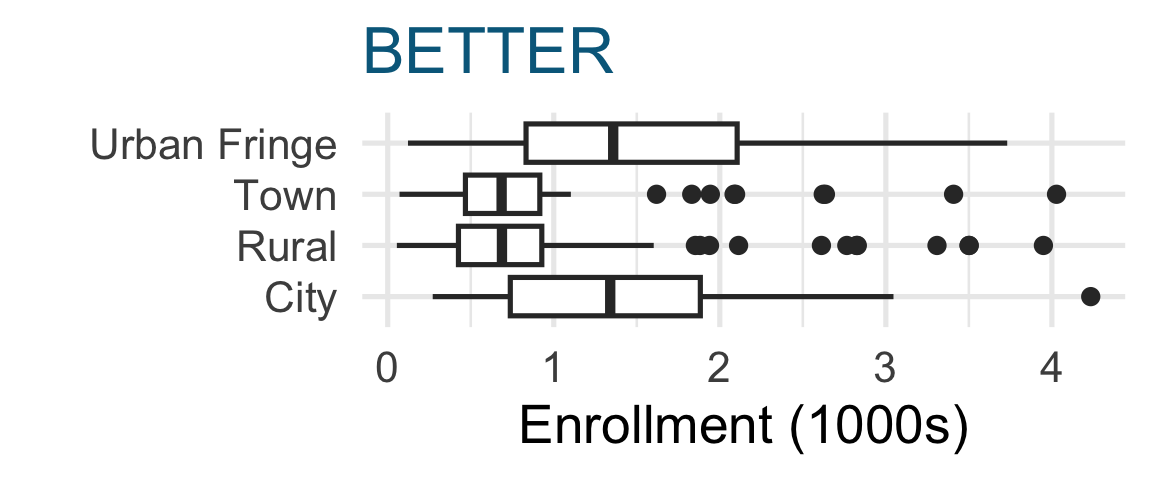
\includegraphics[keepaspectratio]{graph-design-text-elements_files/figure-pdf/also-better-labels-1.pdf}}
\end{center}

\begin{center}
\pandocbounded{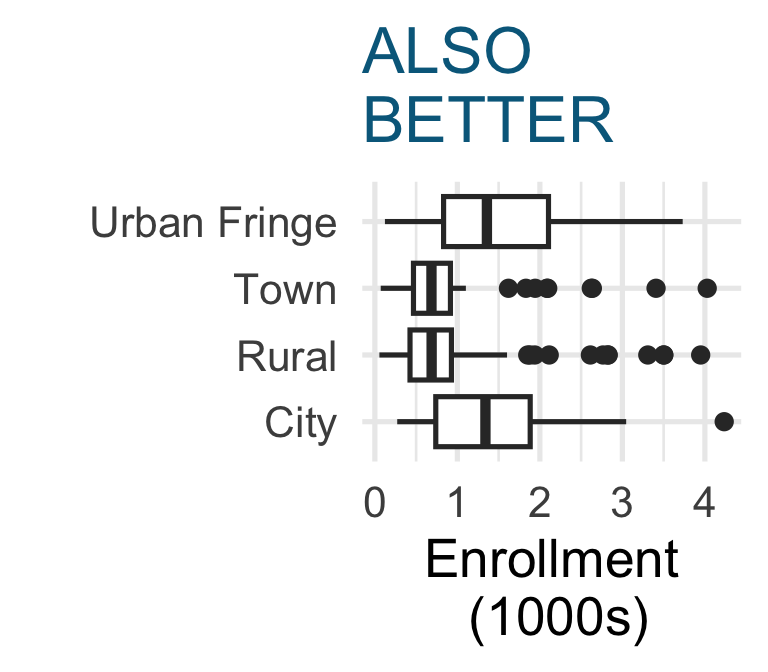
\includegraphics[keepaspectratio]{graph-design-text-elements_files/figure-pdf/better-labels-1.pdf}}
\end{center}

\section{Let's Talk About Titles}\label{lets-talk-about-titles}

Should your graph have a title?

Well\ldots{}\emph{maybe.}

Hear me out.

Whether or not titles are useful, allowed, or expected is pretty
discipline- and audience-specific. In journalism and some parts of
business, they are used very often. In the peer-reviewed scientific
literature, they are exceedingly rare. In a slide deck, they are often
useful\ldots unless they say the same thing as your slide title! Know
your goals and your audience.

\subsection{Avoid Redundant Titles}\label{avoid-redundant-titles}

If you do want to use a title, make \emph{sure} it provides information
or details that are \emph{not} already present in other text elements. A
title that restates the axis labels is usually a waste:

\begin{center}
\pandocbounded{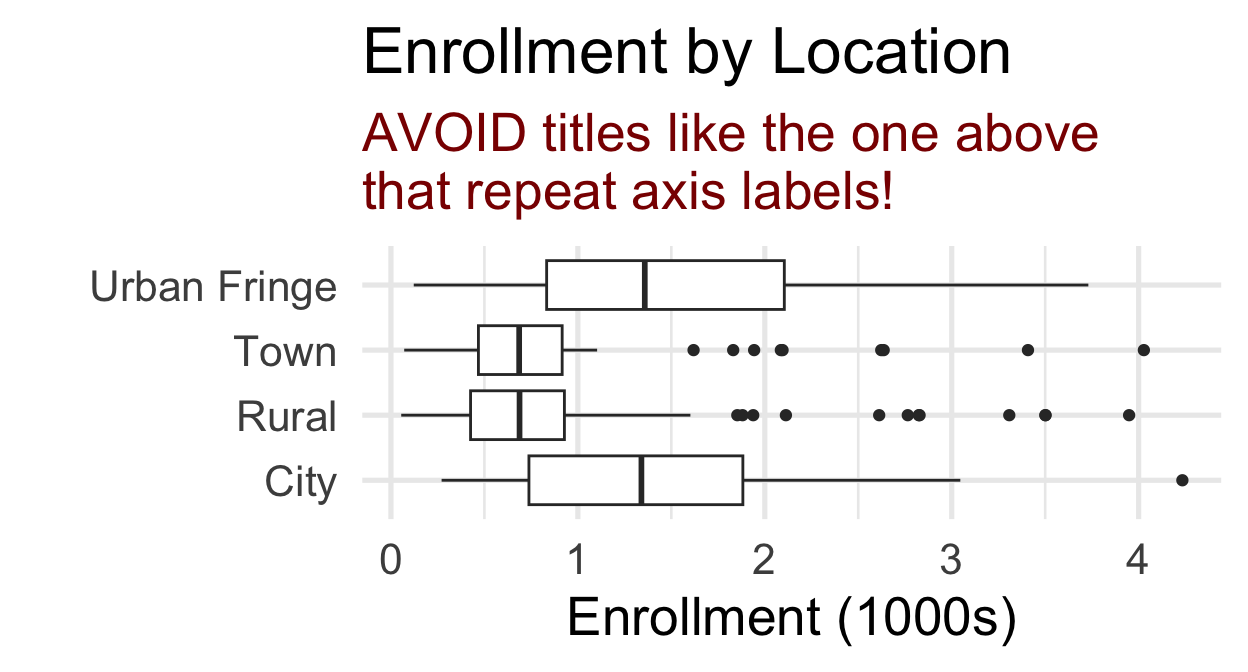
\includegraphics[keepaspectratio]{graph-design-text-elements_files/figure-pdf/bad-title-1.pdf}}
\end{center}

Notice that we can argue about this a little. Could we have the title
\emph{instead} of the axis labels? Maybe, but if it's a scientific
publication, having the units of measure is going to be important.

Is this title \emph{actually adding info} because it clarifies that
``Town,'' ``City,'' etc. are ``Locations''? I think it's a stretch, but
sometimes you can make such a case.

Generally, my advice is\ldots{}

\begin{quote}
\begin{quote}
If the title is not adding something \emph{new and crucial} and helping
the reader decipher the main \emph{story} of the plot, then omit it!
\end{quote}
\end{quote}

So what might an ``informative'' title look like?

\begin{center}
\pandocbounded{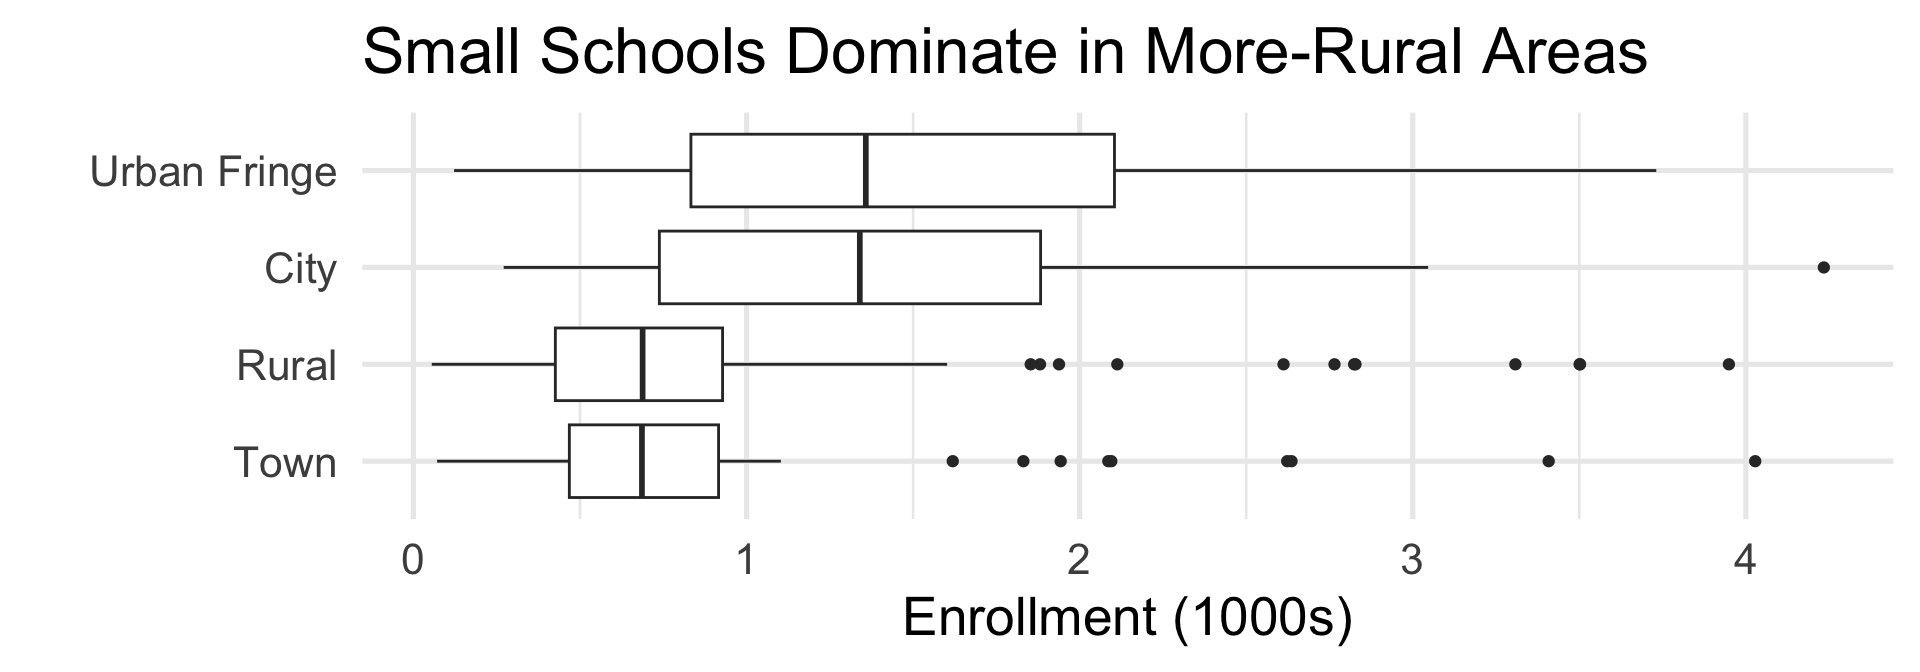
\includegraphics[keepaspectratio]{graph-design-text-elements_files/figure-pdf/ok-title-1.pdf}}
\end{center}

\chapter{Summary}\label{summary}

After reviewing the preceding sections, you should be able to articulate
some principles for designing good visualizations with respect to use of
space, axis limits, use of color, and text elements.

In fact, you probably already \emph{knew} these principles - at least,
you knew 'em when you saw 'em (you could have easily sorted some
terrible and better graphs even if you couldn't have said \emph{exactly}
what was terrible, or better, about them).

Now, think about how you could apply these principles in your own work,
or in providing feedback or advice to others\ldots{}

\section{Critique Practice}\label{critique-practice}

Try using what you have learned to provide a \emph{constructive}
critique of an example. That might mean pointing out specific successes
or positives as well as areas for improvement, with concrete advice
about how to improve and why.

Consider the graphic below. At a glance, what do you think it means?
Looking more carefully, what do you notice?

\includegraphics[width=3.125in,height=\textheight,keepaspectratio]{index_files/mediabag/stand_your_ground.png}

\textbf{Pause to think: What changes, if any, would you suggest to the
figure's creator to make it clearer and easier to understand? Be sure to
be constructive - gently explain any problems and suggest solutions.}

\section{Video Review}\label{video-review}

Wow, that was quite a lot of information! If you could use a brief
review from a different point of view, check out the \textbf{optional}
\href{https://www.youtube.com/watch?v=m9AhRIh49eU}{video from Kristen
Sosulski}

\section{Recap \& Reflect: 12 Tips}\label{recap-reflect-12-tips}

The 4-minute video below summarizes design principles for data
visualization in the form of 12 tips.

As you watch, make note of one or two tips that strike you (you'll
report your thoughts in the next section). Is there one that nicely
summarizes an idea introduced earlier in the section? One you're not
sure about? One that you think is incredibly important? One that makes
you say ``Aha! \emph{Now} I see why I loved/hated that visualization!''

\subsection{Pause for Reflection}\label{pause-for-reflection}

Take a moment to reflect on what you learned. Which Tip do you remember
most clearly, think is most important, or want to challenge? Consider
making a few notes for yourself for the future (you'll have to make and
critique plenty of graphics in your homework assignments).

\section{A Critique Checklist}\label{a-critique-checklist}

If working to improve your own visualization or attempting to give
feedback on one another analyst made, you might consider using a
checklist to guide you.

Based heavily on the advice and template provided by
\href{https://stephanieevergreen.com/data-visualization-checklist/}{Evergreen
Data}\ldots{}

\begin{quote}
\begin{quote}
Check out our
\href{https://stacyderuiter.github.io/stat245-sp25/GraphicsCritiqueChecklist.pdf}{Graphics
Critique Checklist}!
\end{quote}
\end{quote}

\part{Choose a Graph Type}

\section*{Section Learning Outcomes}\label{section-learning-outcomes-1}
\addcontentsline{toc}{section}{Section Learning Outcomes}

\markright{Section Learning Outcomes}

After this tutorial, you will:

\begin{enumerate}
\def\labelenumi{\arabic{enumi}.}
\tightlist
\item
  Distinguish variable types: quantitative, categorical (nominal,
  ordinal, interval, ratio); explanatory, response, covariate.
\item
  Choose an appropriate graphical display for a specified combination of
  variables.
\item
  (Continue to) critique statistical graphics based on design
  principles.
\end{enumerate}

\textbf{Note: You do NOT have to memorize all the information in this
tutorial. Review it now, but know you will probably return to this
tutorial for later reference. Your goal should be to finish with a basic
idea of which graph types should be used for which variable types.
Notice that the ``Gallery'' sections in the navigation bar are labeled
by which variable types are to be shown!}

At the end, you might want to finish with your own notes filling in a
table like the one below:

\begin{longtable}[]{@{}ll@{}}
\toprule\noalign{}
Variables & Graphs \\
\midrule\noalign{}
\endhead
\bottomrule\noalign{}
\endlastfoot
One Quantitative & histogram, density plot, \ldots{} \\
One Categorical & \ldots{} \\
\ldots{} & \ldots{} \\
\end{longtable}

\section*{Text Reference}\label{text-reference}
\addcontentsline{toc}{section}{Text Reference}

\markright{Text Reference}

\begin{itemize}
\tightlist
\item
  \href{https://bookdown.org/roback/bookdown-BeyondMLR/ch-MLRreview.html\#explorech1}{\emph{Beyond
  Multiple Linear Regression} Ch. 1.5}
\item
  \emph{Ecological Models \& Data in R} Ch. 2 discusses graphics, but is
  not recommended as the approach to reading in data, writing R code,
  and generating graphs in R is very different to that used in this
  course.
\item
  A comprehensive, and free, supplemental reference is
  \href{https://clauswilke.com/dataviz/}{Fundamentals of Data
  Visualization by Claus Wilke}
\end{itemize}

\section*{Motivation: Imagine First!}\label{motivation-imagine-first-1}
\addcontentsline{toc}{section}{Motivation: Imagine First!}

\markright{Motivation: Imagine First!}

Figures are a crucial tool for exploring your data \emph{and}
communicating what you learn from the data.

Whether you are doing a quick check to assess basic features of a
dataset or creating a key figure for an important presentation, the best
practice is to work thoughtfully. You already learned about creating
graphics by I.C.E.E:

\subsection*{\texorpdfstring{The \textbf{I.C.E.E.
method}:}{The I.C.E.E. method:}}\label{the-i.c.e.e.-method-1}
\addcontentsline{toc}{subsection}{The \textbf{I.C.E.E. method}:}

\begin{itemize}
\tightlist
\item
  \textbf{I}\emph{magine} how you want your graph to look, \emph{before}
  you
\item
  \textbf{C}\emph{ode}. Once you have the basic starting point,
\item
  \textbf{E}\emph{valuate} your work, and
\item
  \textbf{E}\emph{laborate} (refine it).
\end{itemize}

Repeat until the figure is as awesome as it needs to be.

\subsection*{Limiting Your Imagination}\label{limiting-your-imagination}
\addcontentsline{toc}{subsection}{Limiting Your Imagination}

There is really no limit to the creative data visualizations you might
dream up.

But there is a set of basic, workhorse graphics that statisticians and
data scientists use most frequently. What are the common options and how
do you choose among them?

The best choice depends on what kind of data you have, and also on what
you want to do with it: what question are your trying to answer? What
story will you tell?

\section*{Goals}\label{goals}
\addcontentsline{toc}{section}{Goals}

\markright{Goals}

Specifically, you will now focus on \textbf{choosing the right type of
visualization for the task at hand.}

Note that the graphs shown in this tutorial are over-simplified versions
- icons, really - with missing labels, huge titles, and huge data
elements. This is intentional, to evoke the look of each plot type
rather than to present actual data.

\chapter{Variable Types}\label{variable-types}

Before designing a graphic, you need some data. Ideally, it will be in a
tidy table, with one row per case and one column per variable.

Different plots may be appropriate, depending on whether the variable
is:

\begin{itemize}
\tightlist
\item
  \emph{Categorical} (either nominal or ordinal) or
\item
  \emph{Quantitative} (interval or ratio)
\item
  Beware categorical variables that are stored using numeric codes: they
  are still categorical!
\item
  \emph{Note:} Variables that take on discrete numeric values can be
  treated as either, depending mainly on whether there are a lot of
  possible values (treat like numeric) or few (treat like categorical)
\item
  Other courses or disciplines may distinguish carefully between ordinal
  and nominal data. We often won't, since we don't learn distinct
  methods for them, but treat both as \emph{categorical}.
\end{itemize}

The video below gives a concise explanation of the different variable
types you need to be able to recognize.

\url{https://youtu.be/eghn__C7JLQ?si=Oozu0Z6p4xTBh64z}

\section{Distributions}\label{distributions}

Sometimes, you need a plot that lets you \emph{see} the
\textbf{distribution} of a single variable:

\begin{itemize}
\tightlist
\item
  What \emph{values} does it take on?
\item
  How \emph{often} does each value occur?
\end{itemize}

Sometimes these graphs present the answer to a scientific question of
interest, but often they are used during exploration or model assessment
to better understand a dataset and:

\begin{itemize}
\tightlist
\item
  Check the data

  \begin{itemize}
  \tightlist
  \item
    Are there lots of missing values?
  \item
    Are missing values encoded as 999 or -1000 or some other impossible
    value, instead of being marked as missing via \texttt{NA}?
  \end{itemize}
\item
  Verify whether the variable's distribution matches expectations (for
  example, symmetry, etc.)
\end{itemize}

\chapter{Gallery: One Categorical
Variable}\label{gallery-one-categorical-variable}

\section{Consider your Audience}\label{consider-your-audience}

To show one categorical variable, we will mainly use bar charts. You
might also consider lollipop/Cleveland dot plots, or pie graphs.

\begin{center}
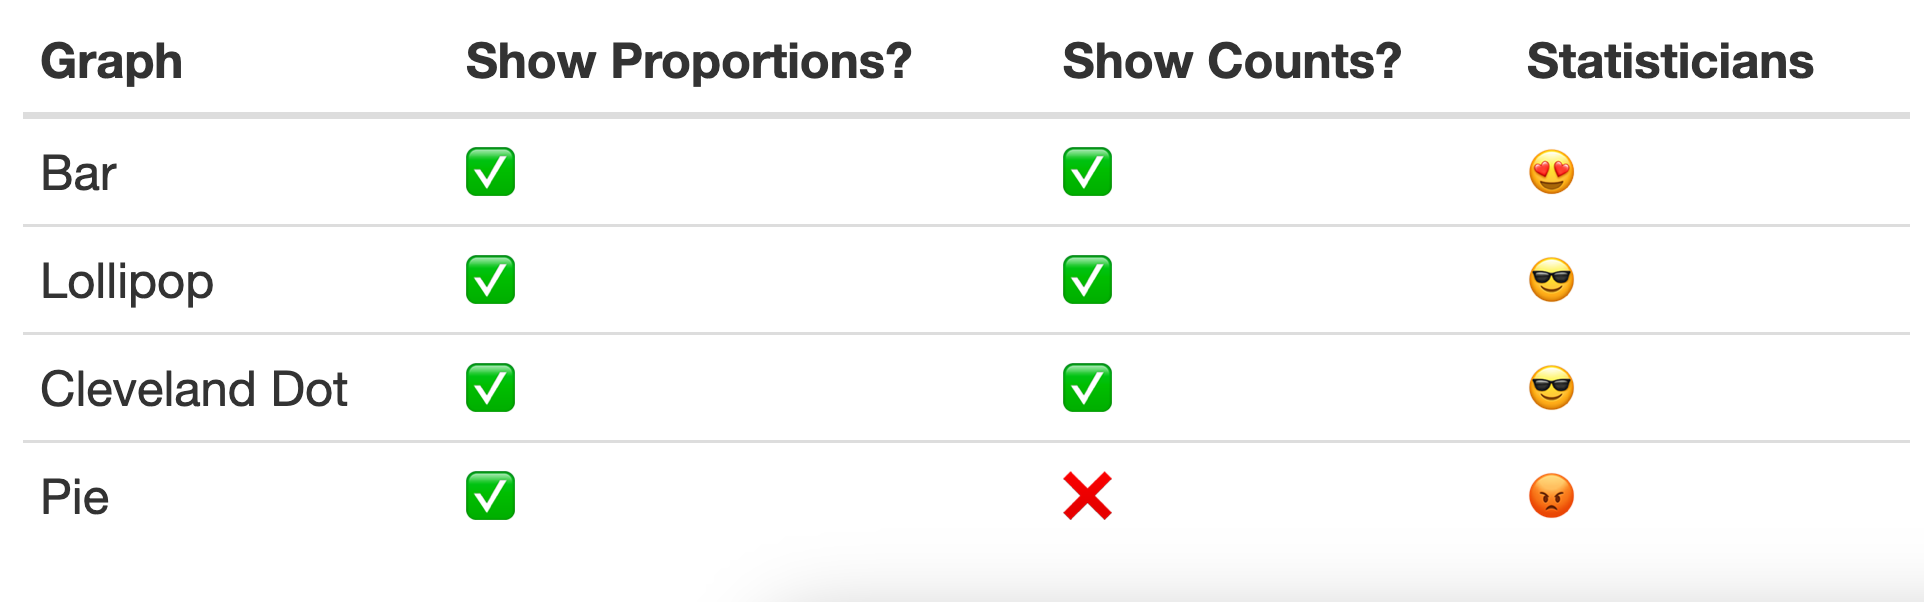
\includegraphics[width=0.8\linewidth,height=\textheight,keepaspectratio]{images/one-cat-emojis.png}
\end{center}

\section{Bar Graph}\label{bar-graph}

\begin{center}
\pandocbounded{\includegraphics[keepaspectratio]{graphics-choose-one-cat_files/figure-pdf/unnamed-chunk-3-1.pdf}}
\end{center}

\begin{itemize}
\tightlist
\item
  Can show either counts, proportions, or percentages
\item
  Easy to see which categories have more/fewer observations
\end{itemize}

\section{Cleveland Dot / Lollipop
Plot}\label{cleveland-dot-lollipop-plot}

\begin{center}
\pandocbounded{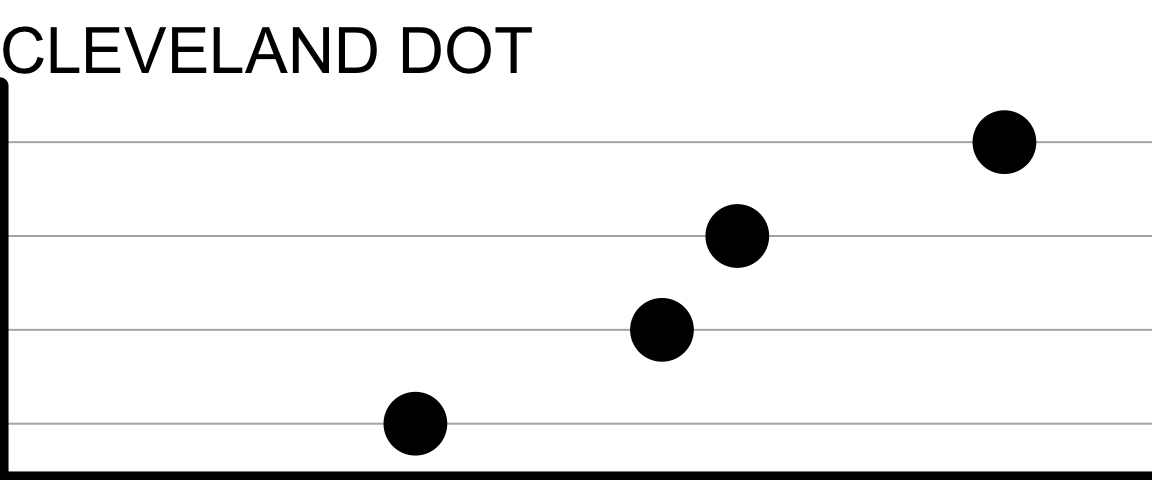
\includegraphics[keepaspectratio]{graphics-choose-one-cat_files/figure-pdf/cleveland-1.pdf}}
\end{center}

\begin{center}
\pandocbounded{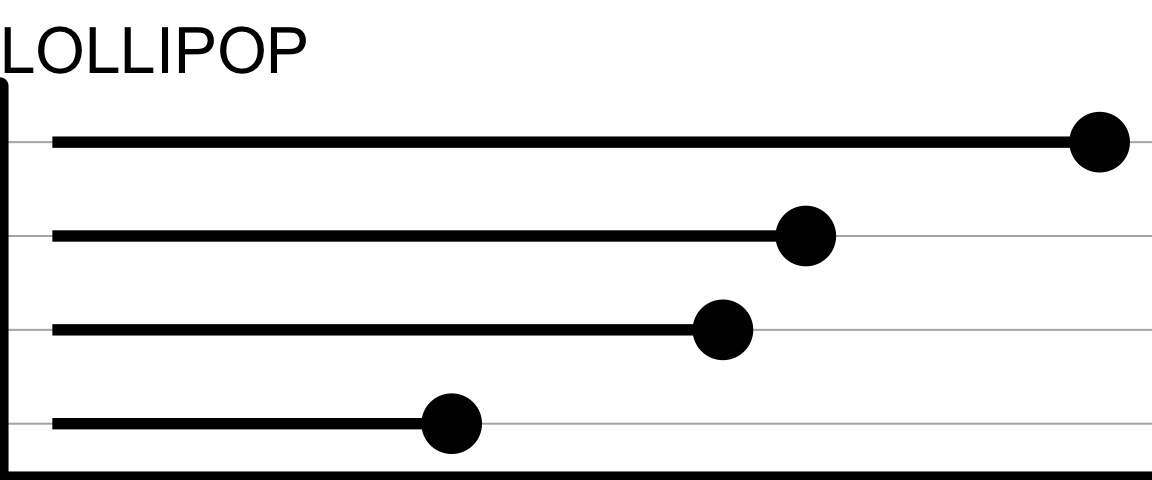
\includegraphics[keepaspectratio]{graphics-choose-one-cat_files/figure-pdf/lollipop-1.pdf}}
\end{center}

\begin{itemize}
\tightlist
\item
  Main difference is whether the ``sticks'' are drawn (Lollipop) or not
  (Cleveland Dot)
\item
  Much like a bar chart, but using dots or lollipops to mark the count
  or proportion in each category
\item
  Work well when there are many categories to be ranked by frequency
\end{itemize}

\section{Pie Chart}\label{pie-chart}

\begin{center}
\pandocbounded{\includegraphics[keepaspectratio]{graphics-choose-one-cat_files/figure-pdf/unnamed-chunk-4-1.pdf}}
\end{center}

\begin{itemize}
\tightlist
\item
  Display proportions, not counts
\item
  Unpopular with many statisticians and data scientists because\ldots{}

  \begin{itemize}
  \tightlist
  \item
    Hard to see which categories have more/fewer observation when
    proportions similar
  \item
    Temptation to clutter them up with annotation (for example,
    percentage for each slice)
  \item
    Can be inefficient use of space on rectangular page
  \end{itemize}
\item
  Often easier to interpret when there are few categories
\end{itemize}

\chapter{Gallery: One Quantitative
Variable}\label{gallery-one-quantitative-variable}

What are some ways to display the distribution of one quantitative
variable?

\section{Dotplot}\label{dotplot}

\begin{center}
\pandocbounded{\includegraphics[keepaspectratio]{graphics-choose-one-quant_files/figure-pdf/unnamed-chunk-2-1.pdf}}
\end{center}

\begin{itemize}
\tightlist
\item
  Intuitive representation: x-axis shows range of variable values, and
  dots are data points
\item
  As the idea is to show one dot per observation, may not work well for
  huge datasets
\end{itemize}

\section{Histogram}\label{histogram}

\begin{center}
\pandocbounded{\includegraphics[keepaspectratio]{graphics-choose-one-quant_files/figure-pdf/unnamed-chunk-3-1.pdf}}
\end{center}

\begin{itemize}
\tightlist
\item
  Range of variable values is divided into bins, then height of each bar
  corresponds to the number of observations in the bin
\item
  Effective way to examine the \emph{shape} of a distribution
\item
  Choosing the number of bins to use is tricky: too many, and the shape
  is jagged; too few over-smooths (peaks blend together). Not sure? Find
  a number of bins that is definitely too few, and one that is
  definitely too many, and then try to settle on an in-between value
  that best shows the real shape of the distribution without
  over-smoothing.
\end{itemize}

\section{Density Plot}\label{density-plot}

\begin{center}
\pandocbounded{\includegraphics[keepaspectratio]{graphics-choose-one-quant_files/figure-pdf/unnamed-chunk-4-1.pdf}}
\end{center}

\begin{itemize}
\tightlist
\item
  Like a smoothed version of a histogram (obtained by kernel density
  estimation, if you want to look up mathematical details)
\item
  Caution: for small datasets, the density plot may show ``peaks'' that
  really correspond to one or a few observations
\item
  Can only show \emph{density} (relative frequency of observation),
  \emph{not counts}
\end{itemize}

\section{QQ Plot}\label{qq-plot}

\begin{center}
\pandocbounded{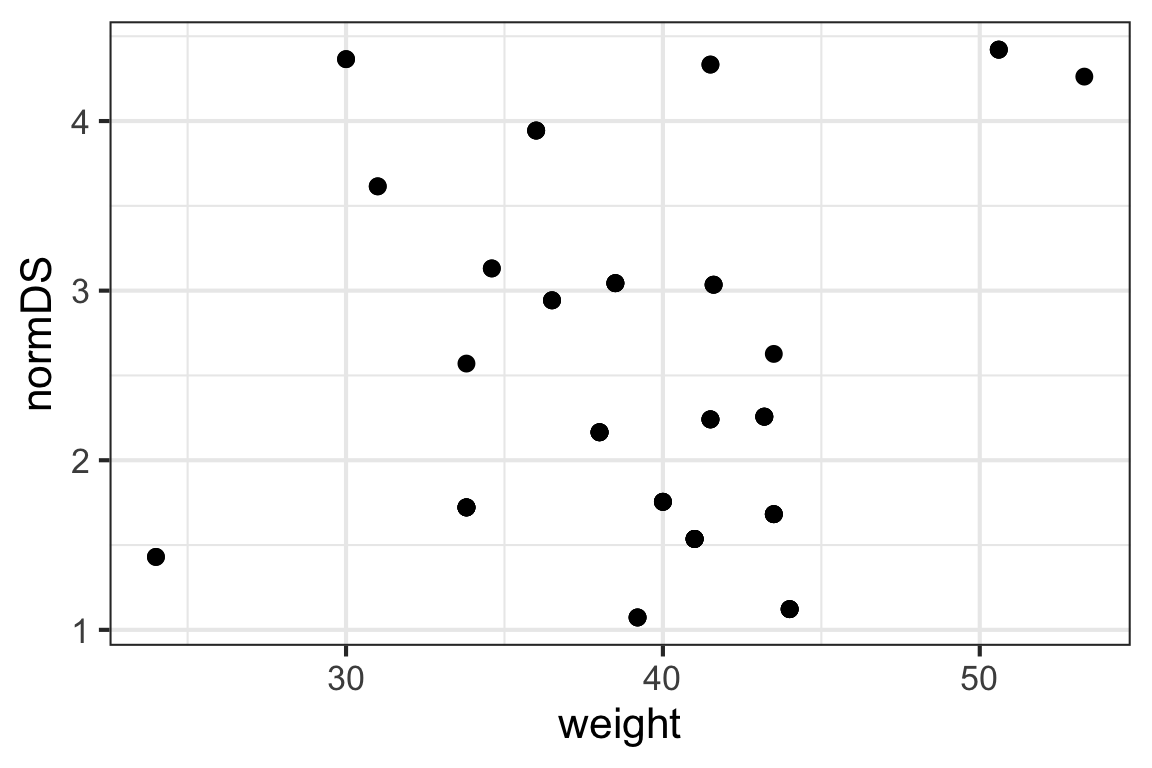
\includegraphics[keepaspectratio]{graphics-choose-one-quant_files/figure-pdf/unnamed-chunk-5-1.pdf}}
\end{center}

\begin{itemize}
\tightlist
\item
  ``Q-Q Plot'' is short for ``Quantile-Quantile Plot''
\item
  In some cases, we want to examine the shape of a variable's
  distribution \emph{to see if it matches a theoretical expectation}.
  For example: do the regression residuals match a normal distribution?
  (If that example doesn't make sense to you now - it will later in the
  course, don't worry.)
\item
  Quantile-quantile plots are one way to make this comparison. They plot
  the quantiles of the data as a function of the same quantiles of the
  expected theoretical distribution; if there's a good match, the points
  should follow a line with slope = 1.
\item
  How close to the straight line is ``close enough''? That's the tricky
  part\ldots{}
\end{itemize}

\section{Check Your Understanding: One-variable
plots}\label{check-your-understanding-one-variable-plots}

Which plot would work best to show the distribution of 75 families'
household incomes?

\begin{itemize}
\tightlist
\item
  \begin{enumerate}
  \def\labelenumi{(\Alph{enumi})}
  \tightlist
  \item
    Lollipop plot\\
  \end{enumerate}
\item
  \begin{enumerate}
  \def\labelenumi{(\Alph{enumi})}
  \setcounter{enumi}{1}
  \tightlist
  \item
    Histogram\\
  \end{enumerate}
\item
  \begin{enumerate}
  \def\labelenumi{(\Alph{enumi})}
  \setcounter{enumi}{2}
  \tightlist
  \item
    Bar chart
  \end{enumerate}
\end{itemize}

Which plot would work best to show the distribution of 75 families'
postal codes?

\begin{itemize}
\tightlist
\item
  \begin{enumerate}
  \def\labelenumi{(\Alph{enumi})}
  \tightlist
  \item
    Bar chart\\
  \end{enumerate}
\item
  \begin{enumerate}
  \def\labelenumi{(\Alph{enumi})}
  \setcounter{enumi}{1}
  \tightlist
  \item
    Density plot\\
  \end{enumerate}
\item
  \begin{enumerate}
  \def\labelenumi{(\Alph{enumi})}
  \setcounter{enumi}{2}
  \tightlist
  \item
    Histogram\\
  \end{enumerate}
\item
  \begin{enumerate}
  \def\labelenumi{(\Alph{enumi})}
  \setcounter{enumi}{3}
  \tightlist
  \item
    Scatter plot\\
  \end{enumerate}
\end{itemize}

Click for explanations of solutions above.

Lollipop plots and bar graphs work better for categorical variables --
they show counts or proportions (or some other summary of counts in
categories). By default, there would be one lollipop or bar for each
unique value of income - what a mess! Histograms and density plots, on
the other hand, show the distribution of one quantitative variable.
(Scatter plots are usually used to show 2 quantitative variables.)

\chapter{Gallery: 2-3 Categorical
Variables}\label{gallery-2-3-categorical-variables}

\begin{center}
\pandocbounded{\includegraphics[keepaspectratio]{graphics-choose-multiple-cat_files/figure-pdf/unnamed-chunk-2-1.pdf}}
\end{center}

\begin{itemize}
\tightlist
\item
  One set of bars per ``category'', colored by ``groups'' -- shows
  \emph{two} categorical variables at once
\item
  Good for showing \emph{counts} in each combination of
  categories/groups
\item
  It is hard to compare proportion in each group across categories, if
  the total number in each category differs.
\end{itemize}

\section{Stacked Bar Graph}\label{stacked-bar-graph}

\begin{center}
\pandocbounded{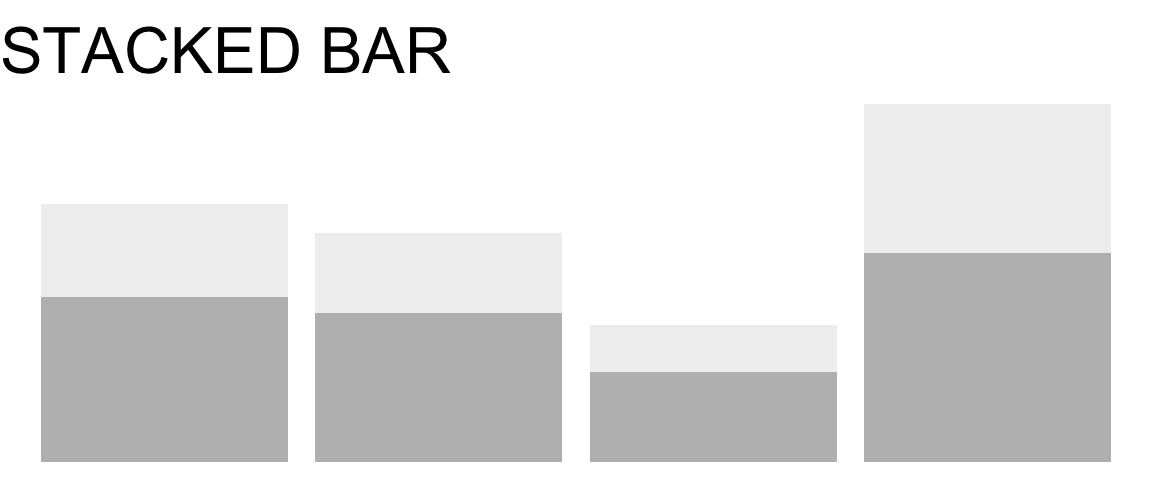
\includegraphics[keepaspectratio]{graphics-choose-multiple-cat_files/figure-pdf/stacked-bar-1.pdf}}
\end{center}

\begin{itemize}
\tightlist
\item
  Similar to side-by-side bar
\item
  Compared to side-by-side, it's \emph{harder} to compare proportions in
  each group within a category, but \emph{easier} to estimate the
  proportion in each category.
\end{itemize}

\section{Faceted Bar Graph}\label{faceted-bar-graph}

\begin{center}
\pandocbounded{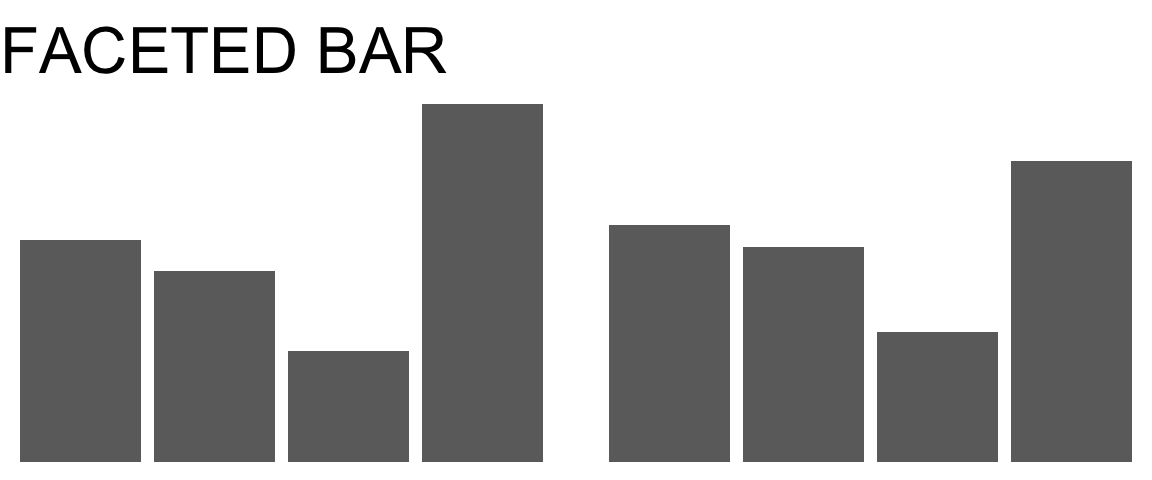
\includegraphics[keepaspectratio]{graphics-choose-multiple-cat_files/figure-pdf/facet-bar-1.pdf}}
\end{center}

\begin{itemize}
\tightlist
\item
  One plot box -- usually called a ``panel'' or ``facet'' -- for each of
  a set of groups
\item
  Think carefully about the question of interest and the relationship
  you want to highlight as you choose: should bar heights correspond
  to\ldots{}

  \begin{itemize}
  \tightlist
  \item
    Number of observations?
  \item
    Proportion of observations \emph{overall in the whole dataset}?
  \item
    Proportion of observations \emph{in the panel}?
  \item
    Something else?
  \end{itemize}
\end{itemize}

\section{Combinations (Stacked bars + Facets,
etc.)}\label{combinations-stacked-bars-facets-etc.}

Of course, if you have 3 variables instead of just two, you \emph{can}
combine methods. Avoid it unless you are sure it is necessary and
communicates clearly.

\begin{itemize}
\tightlist
\item
  \textbf{Be sure that the resulting graph is not too complex to
  understand quickly, at a glance.} Packing too much information into
  one graph sometimes means \emph{none} of the info is actually
  communicated!
\item
  And if showing proportions or percentages in such a display,
  \textbf{be sure you understand what denominator is being used in the
  calculations} -- is it the fraction of the whole dataset, within
  facets, etc.?
\end{itemize}

\begin{center}
\pandocbounded{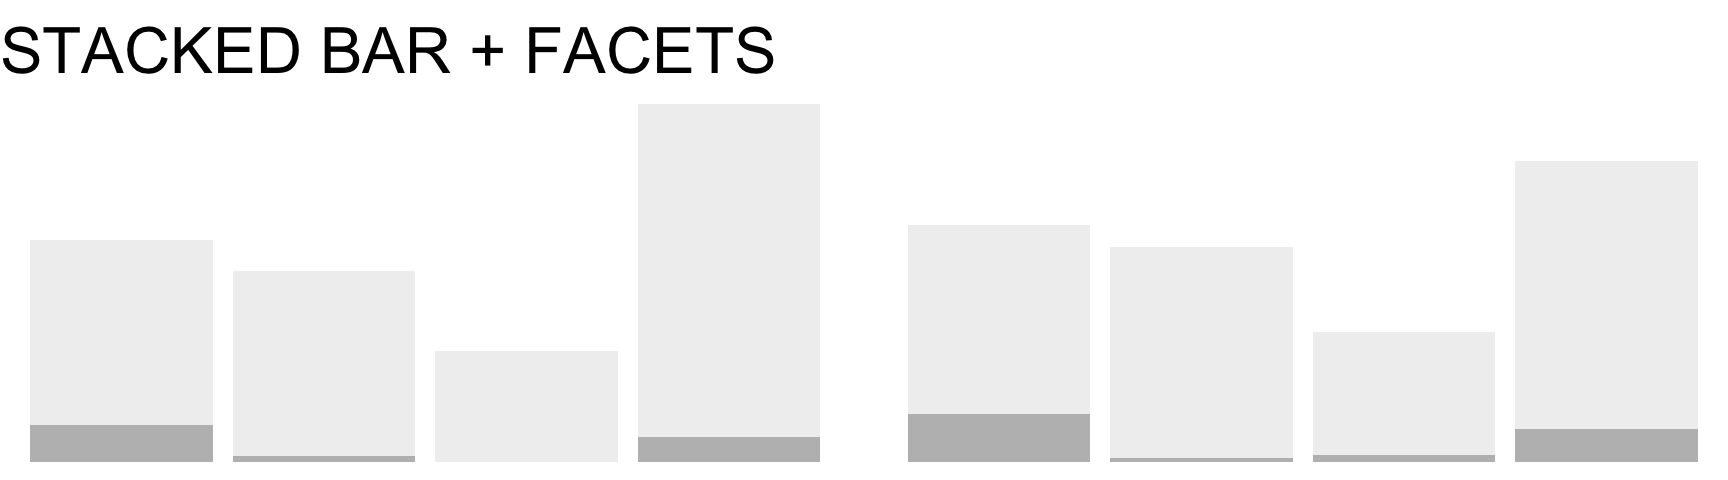
\includegraphics[keepaspectratio]{graphics-choose-multiple-cat_files/figure-pdf/stacked-and-facetted-bar-1.pdf}}
\end{center}

\begin{center}
\pandocbounded{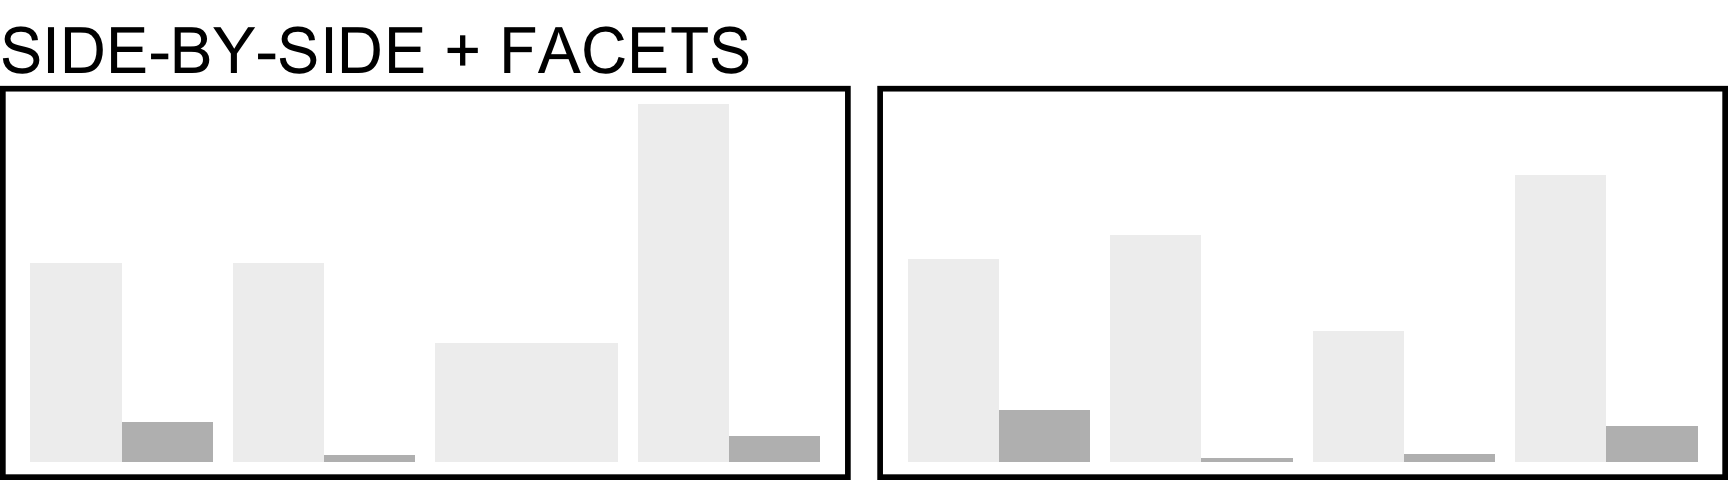
\includegraphics[keepaspectratio]{graphics-choose-multiple-cat_files/figure-pdf/side-by-side-and-facetted-bar-1.pdf}}
\end{center}

\chapter{Gallery: Multiple Quantitative
Variables}\label{gallery-multiple-quantitative-variables}

\section{Scatter Plot}\label{scatter-plot}

\begin{center}
\pandocbounded{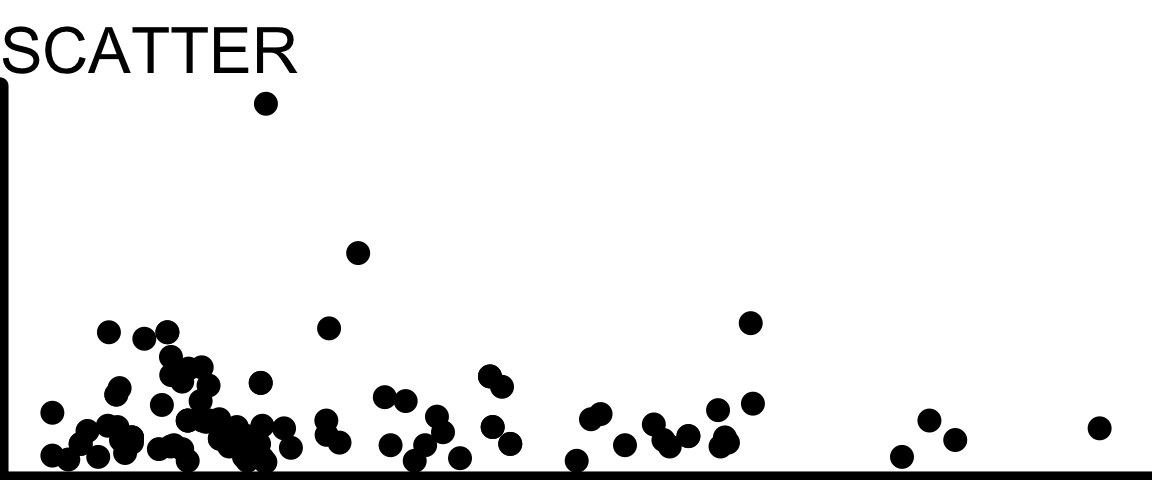
\includegraphics[keepaspectratio]{graphics-choose-multiple-quant_files/figure-pdf/scatter-1.pdf}}
\end{center}

\begin{itemize}
\tightlist
\item
  A scatterplot is the default for visualizing the relationship between
  two quantitative variables
\item
  Be sure you actually have \emph{two quantitative variables}! If not,
  another plot may be a better option.
\end{itemize}

\begin{quote}
\begin{quote}
Let's just reiterate: if one of your variables is \emph{actually} or
\emph{effectively} categorical, a basic scatterplot is usually not
ideal!
\end{quote}
\end{quote}

\section{Line Plot}\label{line-plot}

\begin{center}
\pandocbounded{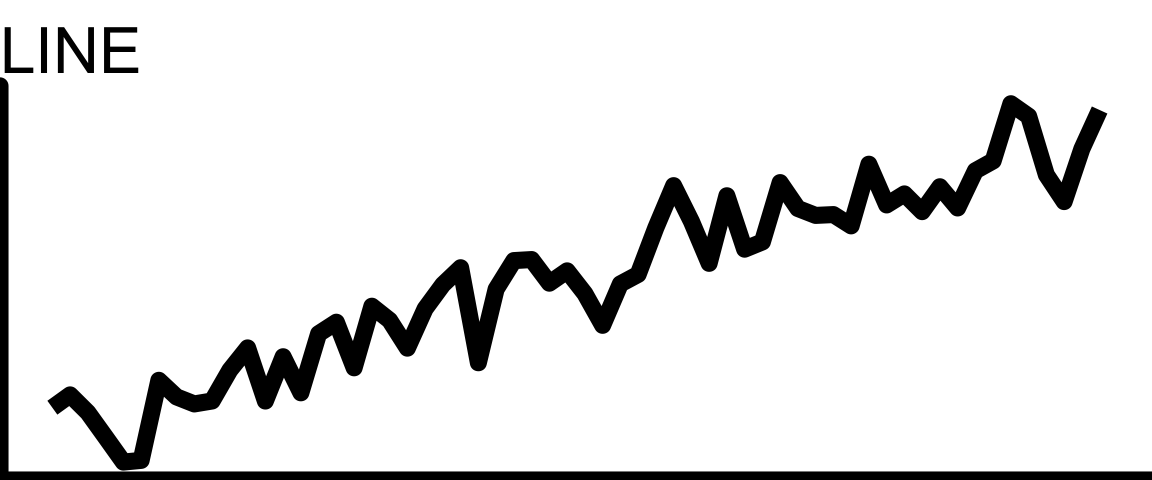
\includegraphics[keepaspectratio]{graphics-choose-multiple-quant_files/figure-pdf/scatter-line-1.pdf}}
\end{center}

\begin{itemize}
\tightlist
\item
  If the x-axis variable is \textbf{Time} (or it otherwise makes sense
  to join the dots), a line can replace the dots, or be added to them
\item
  Make sure connecting the dots makes sense in context and does not
  guide the eye to incorrect interpretations (for example, emphasizing
  outliers)
\end{itemize}

\section{\textgreater2 Quantitative
Variables}\label{quantitative-variables}

What if you have three or four quantitative variables whose
relationships you're curious about?

\emph{Proceed with caution!}

It's possible to include 3+ variables on one plot, but ideally
\textbf{it should still be interpretable at a glance:}

\begin{itemize}
\tightlist
\item
  What is the main point of the figure? Is it possible to make the point
  without showing all 3+ variables together?
\item
  Keep things as simple as you can while still telling the story you
  want to tell.
\end{itemize}

\subsection{Scatter + Size}\label{scatter-size}

\begin{center}
\pandocbounded{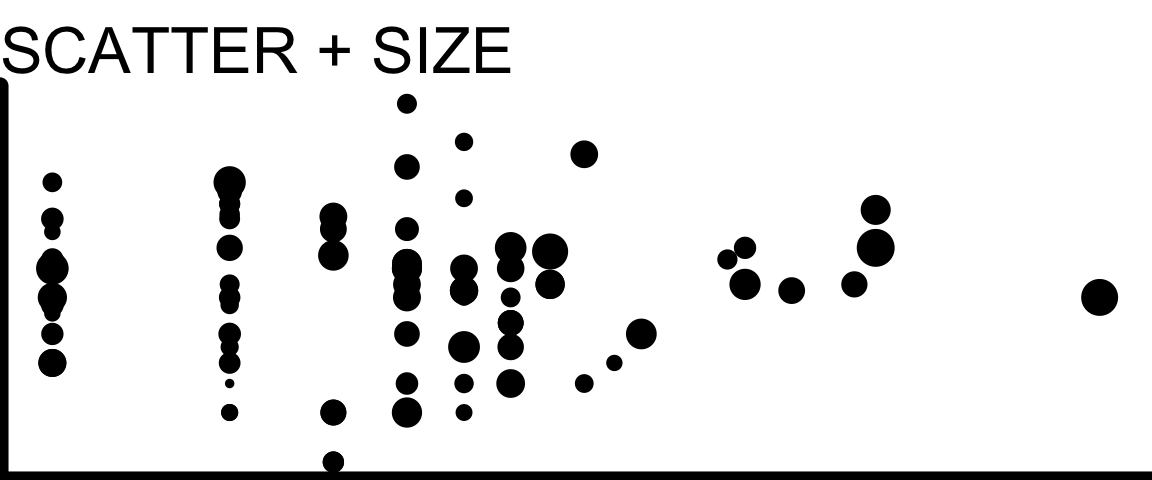
\includegraphics[keepaspectratio]{graphics-choose-multiple-quant_files/figure-pdf/scatter-with-size-1.pdf}}
\end{center}

\begin{itemize}
\tightlist
\item
  You can adjust the size of each dot in a scatter plot to correspond to
  the value of a third variable
\item
  This is especially useful when the third variable measures the size of
  the population being represented -- for example, a scatter plot of
  life expectancy vs income for many countries, with point size
  indicating population of each country
\end{itemize}

\subsection{Scatter + Color}\label{scatter-color}

You can also color by a third quantitative variable:

\begin{center}
\pandocbounded{\includegraphics[keepaspectratio]{graphics-choose-multiple-quant_files/figure-pdf/scatter-with-color-1.pdf}}
\end{center}

This usually only works well visually if all three variables are clearly
associate with each other, so that certain colors are clearly dominant
in certain regions of the graph. Otherwise, you get a mishmash of colors
all over, which can be distracting.

\subsection{Animation}\label{animation}

It may be possible to show a third quantitative variable via animation
(this often works especially well if that third variable is actually
time!)

\begin{center}
\pandocbounded{\includegraphics[keepaspectratio]{graphics-choose-multiple-quant_files/figure-pdf/scatter-with-animation-1.pdf}}
\end{center}

\chapter{Gallery: Mixed Quantitative +
Categorical}\label{gallery-mixed-quantitative-categorical}

\section{Distribution by Groups}\label{distribution-by-groups}

There are several plots designed specifically to look at the
distribution of a quantitative variable, grouped by a categorical
variable.

\subsection{Boxplots}\label{boxplots}

\begin{center}
\pandocbounded{\includegraphics[keepaspectratio]{graphics-choose-cat-quant-mix_files/figure-pdf/boxplot-1.pdf}}
\end{center}

\begin{center}
\pandocbounded{\includegraphics[keepaspectratio]{graphics-choose-cat-quant-mix_files/figure-pdf/boxplot-horiz-1.pdf}}
\end{center}

\begin{itemize}
\tightlist
\item
  The boxplot shows a \emph{summary} of the distribution. The box spans
  the middle half of the data, with the line marking the median. The
  ``whisker'' lines extend to cover the range of ``most of'' the data,
  with outliers shown individually
\item
  For details, check out
  \href{https://openintro-ims.netlify.app/explore-numerical.html\#boxplots}{this
  optional explanation of how boxplots are constructed} from
  \href{https://openintro-ims.netlify.app/index.html}{Introduction to
  Modern Statistics} by Mine Çetinkaya-Rundel and Johanna Hardin.
\item
  If your dataset is too small to estimate the median and quartiles of
  the data accurately, consider showing all the observations (for
  example, using or overlaying a jitter plot)
\end{itemize}

\subsection{Violin Plots}\label{violin-plots}

\begin{center}
\pandocbounded{\includegraphics[keepaspectratio]{graphics-choose-cat-quant-mix_files/figure-pdf/violin-1.pdf}}
\end{center}

\begin{center}
\pandocbounded{\includegraphics[keepaspectratio]{graphics-choose-cat-quant-mix_files/figure-pdf/violin-horiz-1.pdf}}
\end{center}

\begin{itemize}
\tightlist
\item
  These show a mirrored density plot for each group
\item
  As for density plots, make sure you have a large enough dataset so
  that the bumps in the density curve don't represent just one or a
  couple of observations
\end{itemize}

\subsection{Jitter Plots}\label{jitter-plots}

\begin{center}
\pandocbounded{\includegraphics[keepaspectratio]{graphics-choose-cat-quant-mix_files/figure-pdf/jitter-1.pdf}}
\end{center}

\begin{itemize}
\tightlist
\item
  These show all the points in every category, ``jittered'' (moved
  slightly away from the category axis) to reduce overplotting
\item
  If the dataset is too large, overplotting may still be a big problem
\item
  Jitter plots are often used as an additional layer on top of boxplots
  or violin plots to make the size of the dataset, and the locations of
  individual datapoints, more visible
\end{itemize}

\subsection{Sina Plots}\label{sina-plots}

\begin{center}
\pandocbounded{\includegraphics[keepaspectratio]{graphics-choose-cat-quant-mix_files/figure-pdf/sina-1.pdf}}
\end{center}

\begin{itemize}
\tightlist
\item
  These show all the points in every category, arranged so that the
  width of the point cloud corresponds to the density of observations
\item
  If the dataset is too large, overplotting may become an issue
\item
  A sina plot is a bit of a hybrid between a violin plot and a jitter
  plot; or, a more organized, less random version of a jitter plot.
\end{itemize}

\section{Facets?}\label{facets}

You can also consider making multi-panel plots with one histogram,
density plot, or dotplot per facet, but comparing between facets is
usually harder than comparing boxplots or violin plots on a single axis.

Multi-facet plots can show one panel per group, for \emph{any} kind of
plot seen so far: a bar graph for each group, a stacked bar for each
group, a scatterplot for each group, a set of boxplots for each group,
etc. etc.

\begin{center}
\pandocbounded{\includegraphics[keepaspectratio]{graphics-choose-cat-quant-mix_files/figure-pdf/facetted-box-1.pdf}}
\end{center}

\subsection{Check Your Understanding: Quant. +
Cat.}\label{check-your-understanding-quant.-cat.}

\textbf{There are some errors and inconsistencies in the chart below!}

Check it out -- can you find them?

\begin{figure}[H]

{\centering \includegraphics[width=6.25in,height=\textheight,keepaspectratio]{index_files/mediabag/chart-types-infograp.png}

}

\caption{chart choice infographic}

\end{figure}%

\bookmarksetup{startatroot}

\chapter*{References}\label{references}
\addcontentsline{toc}{chapter}{References}

\markboth{References}{References}

\phantomsection\label{refs}
\begin{CSLReferences}{0}{1}
\end{CSLReferences}




\end{document}
